\documentclass[11pt,a4paper]{report}

\usepackage[english]{babel}
\usepackage[utf8]{inputenc}
\usepackage{amsmath}
\usepackage{graphicx, rotating}
\usepackage[margin=1in]{geometry}
\geometry{left=1.2in, right=0.8in}
\usepackage{subfigure}

%fancy headers
\usepackage{fancyhdr}
\pagestyle{fancy}{
	\fancyhf{} % clear all header fields
	\fancyhead[LO,RE]{\leftmark}
	\fancyhead[LE,RO]{\thepage}}


\renewcommand{\headrulewidth}{0.8pt}

%introduces penalties for widows and orphans
\widowpenalty10000
\clubpenalty10000

\usepackage{parskip} %avoids indents on each new paragraph
\usepackage{float}  %allows me to place figures where I write them
\usepackage[printonlyused]{acronym} %creates a list of acronyms
\usepackage{lscape} %allows me to turn sections of text landscape
%line spacing commands
\renewcommand{\baselinestretch}{1.5}
\usepackage{setspace}
\usepackage{wrapfig, float} %lets text wrap around tables
%packages to do with the subfigure option
\usepackage{caption}
\usepackage{dcolumn}
\usepackage{amssymb} %for checkmarks in tables
\usepackage{array}
\usepackage{tabularx} %for table editing
\usepackage{listings} %to write R code
\usepackage{ragged2e} %justified text

\usepackage{enumitem} %reducing space around lists
\setlist{nosep} % or \setlist{noitemsep} to leave space around whole list

\usepackage[backend=bibtex, style=ieee]{biblatex}
\addbibresource{bibl.bib}

\usepackage{xcolor}
\definecolor{light-gray}{gray}{0.95}

\begin{document}


\begin{titlepage}
	
	\newcommand{\HRule}{\rule{\linewidth}{0.5mm}} % Defines a new command for the horizontal lines, change thickness here
	
	\center % Center everything on the page
	%----------------------------------------------------------------------------------------
	%	LOGO SECTION
	%----------------------------------------------------------------------------------------
	
	\includegraphics[scale=0.2]{images/logo.jpg}\\[1cm] % Include a department/university logo - this will require the graphicx package
	
	%----------------------------------------------------------------------------------------
	\vspace{0.4cm}
	%----------------------------------------------------------------------------------------
	%	HEADING SECTIONS
	%----------------------------------------------------------------------------------------
	
	\textsc{\LARGE Cardiff University}\\[1.5cm] % Name of your university/college
	\textsc{\Large BSc Mathematics and its Applications}\\[0.5cm] % Major heading such as course name
	\textsc{\large Final Year Project}\\ % Minor heading such as course title
	
	
	\vspace{1cm}
	%----------------------------------------------------------------------------------------
	%	TITLE SECTION
	%----------------------------------------------------------------------------------------
	\vspace{1.5cm}
	\HRule \\[0.4cm]
	{ \huge \bfseries Modelling the National Student Survey to Predict Overall Satisfaction}\\[0.4cm] % Title of your document
	\HRule \\[1.5cm]
	
	%----------------------------------------------------------------------------------------
	%	AUTHOR SECTION
	%----------------------------------------------------------------------------------------
	
	\begin{minipage}{0.4\textwidth}
		\begin{flushleft} \large
			Nina \textsc{Di Cara}\\
			c1210839 % Your name
		\end{flushleft}
	\end{minipage}
	~
	\begin{minipage}{0.4\textwidth}
		\begin{flushright} \large
			\emph{Supervised by:} \\
			Dr. Jonathan \textsc{Gillard} % Supervisor's Name
		\end{flushright}
	\end{minipage}\\[4cm]
	
	% If you don't want a supervisor, uncomment the two lines below and remove the section above
	%\Large \emph{Author:}\\
	%John \textsc{Smith}\\[3cm] % Your name
	
	%----------------------------------------------------------------------------------------
	%	DATE SECTION
	%----------------------------------------------------------------------------------------
	
	{\large May 2016}\\[3cm] % Date, change the \today to a set date if you want to be precise
	
	
	\vfill % Fill the rest of the page with whitespace
	
\end{titlepage}


\thispagestyle{empty}
\begin{centering}
{\large \bfseries{Acknowledgements}} \\
\end{centering}
\vspace{1cm}
I would like to express my great appreciation to Dr. Gillard for his excellent guidance, advice and support during the writing of this project. 

My special thanks are also extended to the staff in Cardiff University's Student Engagement Team, as the opportunity to complete this project is largely due to the warmth and support I received, and still receive, as part of this team. 

Additionally I would acknowledge the support of my family and friends both in completing this project, and throughout my university career, for which I am extremely grateful. 

\begin{abstract}
	In Higher Education students are frequently surveyed throughout their time at university through various national surveys, headed by funding bodies. With increasing focus from the Quality Assurance Agency for departments to achieve positive results in these surveys, and the results reported for the public to view there is real pressure on institutions to satisfy their students. This report looks in detail at the National Student Survey, which assesses the satisfaction of final undergraduate students in a range of areas, and asks them to rate their Overall Satisfaction; the particular focus was to understand which of the other survey items may indicate a high level of Overall Satisfaction, and thus which could be targeted by universities to increase student satisfaction. In order to do this 10 years of NSS data were analysed using multiple regression, and then multilevel modelling, from which several recommendations were made as to modelling this data in the future. The results indicated that good organisation and management of the course was by far the most important predictor of Overall Satisfaction, and following closely were two questions on teaching, namely that staff are good at explaining things and that the course is intellectually stimulating. 
\end{abstract}


\tableofcontents
\thispagestyle{empty}
\addtocontents{toc}{\protect\thispagestyle{empty}} %supresses numbering on both pages of toc



\newpage
\setcounter{page}{1}
\thispagestyle{plain}
{\huge \textbf{Acronyms}}

\vspace{0.5cm}

{\large \textbf{Survey and Higher Education Acronyms}}
\begin{acronym}
	\addcontentsline{toc}{chapter}{Acronyms}
	\acro{CEQ}{Course Experience Questionnaire}
	\acro{DAP}{Degree Awarding Powers}
	\acro{DHLE}{Destination of Leavers of Higher Education}
	\acro{HE}{Higher Eduction}	
	\acro{HEA}{Higher Education Academy}
	\acro{HEFCE}{Higher Eduction Funding Council for England}
	\acro{HEFCW}{Higher Eduction Funding Council for Wales}	
	\acro{HEI}{Higher Education Institution}
	\acro{HESA}{Higher Education Statistics Agency}
	\acro{ISB}{International Student Barometer}
	\acro{JACS}{Joint Academic Coding System}
	\acro{NSS}{National Student Survey}
	\acro{OS}{Overall Satisfaction}
	\acro{PRES}{Postgraduate Research Experience Survey}
	\acro{PTES}{Postgraduate Taught Experience Survey}
	\acro{QAA}{Quality Assurance Agency}
	\acro{UCAS}{Universities and Colleges Admissions Service}
	\acro{UKES}{United Kingdom Engagement Survey}
\end{acronym}
\vspace{0.8cm}
{\large \textbf{Statistical Acronyms}}
\begin{acronym}
	\acro{AIC}{Akaike's Information Criterion}
	\acro{ANOVA}{Analysis of Variance}
	\acro{BIC}{Schwarz's Bayesian Criterion}	
	\acro{CV}{Cross-Validation}
	\acro{EBLUP}{Estimated Best Least Unbiased Predictors}
	\acro{ICC}{Intra-Class Correlation Coefficient}	
	\acro{ML}{Maximum Likelihood}
	\acro{MSPE}{Mean Square Predicion Error}
	\acro{REML}{Restricted Maximum Likelihood}
	\acro{RMSPE}{Root Mean Square Prediction Error}
	\acro{VIF}{Variance Inflation Factor}
\end{acronym}


\chapter{Introduction}
\section{Student Surveys in the UK}
The number of surveys of students in \ac{HE} has steadily increased over the past 10 years, and currently there are a number of an annual national \ac{CEQ} being used to benchmark student experience, from those students entering university to postgraduate researchers. These surveys include the \ac{PRES}, \ac{PTES} and \ac{UKES} run by the \ac{HEA} \cite{HEASurveysPage}, the \ac{DHLE} owned by the \ac{HESA} \cite{DLHEPage} as well as the \ac{ISB} which is run internationally \cite{ISBPage}. Perhaps the most well known and widely reported student survey is the \ac{NSS} \cite{NSSsite}.

For students, there is undeniable value in these evaluations of their experiences. Surveys are one of the most convenient and accessible ways for students to share their views with senior management, with universities held to account by organisations such as the \ac{QAA} \cite{QualityCode} to prove that they are acting on student suggestions. As well as being examined in internal and external quality assurance procedures the results of many surveys are open to public scrutiny, even reported in  the national press \cite{2015NSSNews},  meaning that `good' results can be essential to maintaining a university's public reputation. The increased attention on the results of student surveys has also led to their integration in league table calculations, with those such as the Complete University Guide, and the Guardian incorporating overall student satisfaction into their league table calculations amongst other NSS measures \cite{CompleteLeague, GuardianLeague}. Additionally, results from the NSS are made publicly available through UniStats \cite{UniStatssite}, a website which provides statistical information on attainment and satisfaction for prospective university students, and it has been shown that a course's NSS scores can have a statistically significant influence on the volume of applications they receive \cite{gibbons2013student} which shows the power that these surveys have.

\section{The National Student Survey}
The \ac{NSS} is a nationwide \ac{CEQ}, undertaken in all publicly funded Higher Education Institutions (HEIs) in the United Kingdom, which has run annually since 2005 \cite{2007initialnss}. It is commissioned by the \ac{HEFCE} on behalf of the \ac{HEFCW} alongside other major funding bodies and is independently run by the polling agency Ipsos MORI \cite{IpsosMoriNSS}, with the results reported by Texunatech \cite{TexunaNSS}. Intended for final year undergraduates, the survey has three main aims: \\
1. To inform student decisions\\
2. To provide information to enhance the student learning experience \\
3. To support quality assurance and accountability.\\
However, even these three simple aims of the survey are a point of contention for academics within HE institutions \cite{child2011perception}. 

The survey uses a 5-point Likert scale of satisfaction with students answering 23 questions, which are grouped as described in Table \ref{table:NSSquestions} in order to cover six aspects of a student's learning experience. 
As well as the six main thematic areas, institutions can also choose to opt into various `banks' of questions which give additional statements around other topics such as learning community, quality of the physical learning environment, and work experience. Students also have the opportunity to give positive and negative written comments at the end of the survey.  

With the increased attention on the \ac{NSS} there have been concentrated efforts to increase the response-rates and gather more accurate information year on year. Sector-wide there has been an upward trend in response since the \ac{NSS} launched in 2006 and the latest figures show that nearly half a million students responded (see Figure \ref{fig:responsetrend}).

\begin{figure}[H]
	\centering
	\includegraphics[scale=0.5]{images/SectorResponseRates.pdf}
	\caption{NSS Sector-Wide Response Rate (\%) By Year}
	\label{fig:responsetrend}
\end{figure}

For many institutions the results of the \ac{NSS} form part of their key performance indicators \cite{NSSpainorgain2009}, and are expected to be used as the basis for enhancement across all areas of their provision. Whilst many staff regard this as a positive opportunity for the student voice to be acknowledged, many academics are disillusioned by the concept \cite{child2011perception} and are not confident in the survey's ability to contribute useful information \cite{NSSworthless2008, AbolishNSS2015}, instead believing that efforts to increase survey results stand in the way of genuinely improving the student experience.\\ 


\begin{table}[p]
	\caption{National Student Survey: Main Question Bank divided by Thematic Area}
	\begin{tabular}{ll} \hline \hline
	\multicolumn{2}{l}{\textbf{Thematic Area 1: Teaching on my course}}  \\[0.1cm]
	Q1. & Staff are good at explaining things \\[0.1cm]
	Q2. &Staff have made the course interesting \\[0.1cm]
	Q3. &Staff are enthusiastic about what they are teaching \\[0.1cm]
	Q4. &The course is intellectually stimulating\\[0.3cm] 

	\multicolumn{2}{l}{\textbf{Thematic Area 2: Assessment and Feedback}}  \\[0.1cm] 
	Q5. &The criteria used in marking have been made clear in advance \\[0.1cm]
	Q6. &Assessment arrangements and marking have been fair \\[0.1cm]
	Q7. &Feedback on my work has been prompt \\[0.1cm]
	Q8. &I have received detailed comments on my work \\[0.1cm]
	Q9. &Feedback on my work has helped me to clarify things I didn't understand\\[0.3cm] 

	\multicolumn{2}{l}{\textbf{Thematic Area 3: Academic Support}} \\[0.1cm]
	Q10. &I have received sufficient advice and support with my studies \\[0.1cm]
	Q11. &I have been able to contact staff when I needed to  \\[0.1cm]
	Q12. &Good advice was available when I needed to make study choices\\[0.3cm] 

	\multicolumn{2}{l}{\textbf{Thematic Area 4: Organisation and Management}} \\[0.1cm]

	Q13. &The timetable worked efficiently as far as my activities are concerned \\[0.1cm]
	Q14. &Any changes in the course or teaching have been communicated effectively \\[0.1cm]
	Q15. &The course is well organised and running smoothly\\[0.3cm] 

	\multicolumn{2}{l}{\textbf{Thematic Area 5: Learning Resources}} \\[0.1cm]

	Q16. &The library resources and services are good enough for my needs \\[0.1cm]
	Q17. &I have been able to access general IT resources when I needed to \\[0.1cm]
	Q18. &I have always been able to access specialised equipment, facilities, rooms when needed\\[0.3cm] 

	\multicolumn{2}{l}{\textbf{Thematic Area 6: Personal Development}} \\[0.1cm]

	Q19. &The course has helped me to present myself with confidence \\[0.1cm]
	Q20. &My communication skills have improved \\[0.1cm]
	Q21. &As a result of the course, I feel confident in tackling unfamiliar problems\\[0.3cm] 

	\multicolumn{2}{l}{\textbf{Thematic Area 7: Overall Satisfaction}} \\[0.1cm]

	Q22. &Overall, I am satisfied with the quality of my course \\[0.1cm]
	\hline \hline
	\end{tabular}
\label{table:NSSquestions}
\end{table}


\section{Research Outline} \label{Research Q}

As a result of the increased pressure on institutions to perform well in the NSS, this research asks \textbf{what are the main predictors of Overall Satisfaction?}

Whilst there are many ways to approach the question, this analysis will be focussed around the data available from the NSS itself and using statistical analyses to uncover subtle relationships between the survey questions and other factors. This data includes the scores from responses from over 400 UK institutions across 10 years from 2006 to 2015 inclusive for all of the main question bank survey items. This is described further in Section \ref{Data}. 

 It is hoped that the scores given for Q1 to Q21 will be indicative of the score for Q22, \ac{OS}. If this can be inferred from the data then it may imply that there are specific areas of a student's education at university where enhancement efforts are more likely to lead to an increased \ac{OS} score in the NSS. Given how widely reported this single score is, and the weight placed on it by prospective students, league tables and the press it is clear why it could be considered the most important survey item to understand.  
 
 As pointed out by many academics \cite{AbolishNSS2015,NSSworthless2008,NSSpainorgain2009}, this may not necessarily be the empirical answer to what student satisfaction is and how to improve it, but it could at least allow further interpretation into what it is and what affects it. 

\newpage
\chapter{Review of the Literature} \label{lit review} 
\section{Statistical Research into the NSS}
Given the aforementioned emphasis on the results of \ac{CEQ}s there is a wide base of research dedicated to finding underlying meaning and information from the rich bank of student opinions they provide. As discussed by Child \cite{child2011perception}, many institutions have realised that the information created for use by the public (such as percentages of satisfaction and question agreement) is not the information which universities find useful for enhancement purposes, a key aim of the \ac{NSS}. Thus there is increasing interest in extracting `useful' information from the \ac{NSS}, and other student surveys, using more sophisticated statistical techniques which probe the latent relationships present in the data in the hope that these will tell institutions what students really want. 

In answer to the desire for deeper understanding of the data many researchers have endeavoured to explore the background contributions to \ac{OS} in \ac{CEQ}s. One of the first ways in which this has been interpreted is by considering student characteristics, such as age, gender and mode of study, and how these explain variance in the data for Overall Satisfaction-type questions. Research from \ac{HEFCE} \cite{surridge2005-2007}, and Marsh and Cheng \cite{marshandcheng2008} into the \ac{NSS}, as well as Denson \cite{denson2010whatpredicts} into an Australian \ac{CEQ} all found that, on average, males rate courses lower than females. As an extension to these findings, the 2005 HEFCE \cite{2007initialnss} report also found that mature students are also more likely to be dissatisfied. 

Whilst this is interesting, both Marsh and Cheng \cite{marshandcheng2008} and Denson \cite{denson2010whatpredicts} also found that student characteristics accounted for a small amount of the variation in Overall Satisfaction, and thus are of little consequence in the interpretation of satisfaction. Denson's research did find that \ac{CEQ}s, like the NSS, accounted for a large part of the variation in student satisfaction, in comparison with motivations for enrolling on the course and student characteristics, which were both ultimately inconsequential \cite{denson2010whatpredicts}. This is an affirmation that \ac{CEQ}s are ultimately useful in providing quality information on what satisfies students. Deeper research into the evaluations themselves has also suggested that of the many topics covered, questions around teaching are the most strongly related to student satisfaction \cite{ginns2007students}.

Another interpretation of the data available is to analyse responses with respect to discipline and institution as well as individual student characteristics; this can be achieved through a statistical technique called multilevel modelling. Multilevel modelling allows data to be analysed with respect to its hierarchical structure, for instance students within classes, within schools. A fuller explanation of this technique may be found in Section \ref{methodMLM}. An attempt to analyse the NSS in this way has been conducted by both Marsh and Cheng \cite{marshandcheng2008} and Hewson \cite{hewson2011preliminary}, who both found notable differences in responses between disciplines, though not between institutions. This was further explored by Cheng \cite{cheng2010unicoursediffs} who found that differences between universities accounted for less than 3\% of the variation in individual student responses, and that far more variation was explained by difference in courses for the 2005-2006 NSS data. The overall recommendation from the paper was that these data should be modelled on three levels (level 1 = students, level 2 = courses, level 3 = university).

The consideration of subtle subject level complexities with respect to OS was also highlighted by Fielding \cite{fielding2010sciencesubjects}, who noted that while universities as a whole may simply attempt to work on their lowest scoring institutional area it is in fact vital to consider differences at subject level in order to fully understand the underlying issues that the data explains. These results point to the crucial importance of considering discipline level information when attempting a more sophisticated analysis of the \ac{NSS} data.

Those papers outlined above all present interesting results, though all only consider either two or three years of data. The first full review of a significant amount of \ac{NSS} data was conducted by \ac{HEFCE} in 2014, during their review of the \ac{NSS} \cite{HEFCEreport2014}. They considered the full set of a data from 2005-2014 of a core set of institutions who had been part of the NSS since it began and investigated the robustness of the survey. Whilst there were many interesting results, such as the differences in ethnicity and other student characteristics, the overall question of what makes students satisfied was not fully explored. 

\section{Summary}
There has been a strong base of research focussed on interpreting student satisfaction as an outcome of \ac{CEQ}s, in different countries and educational scenarios and several messages can be taken from what has been found. The following summary points are those which are considered important in the context of the research being undertaken in this project:
\begin{itemize}
	\item student characteristics account for only a small amount of the variation in \ac{OS},
	\item discipline information is an important factor when analysing \ac{OS},
	\item discipline information accounts for more variation in student responses than institution level information,
	\item multilevel modelling can be conducted on NSS data, structured as student, within course, within institution,
	\item \ac{OS} has not been rigorously examined with respect to the other NSS questions in order to predict overall satisfaction on more than three years of data, 
	\item questions around teaching have been suggested as a key predictor of student satisfaction.
\end{itemize}

Given this information, this research intends to use all available previous NSS data from the years 2005 to 2015 in order to analyse \ac{OS} with respect to the other survey questions and investigate whether teaching questions are indeed a key predictor of student satisfaction, and what the effects are of modelling the data on multiple levels.

\newpage
\chapter{The Data} \label{Data}
%inital plots of the data and the basic descriptions of the data
%including: pie charts, bar charts, box plots of outliers
This chapter describes the data used in the analyses ahead, how it was obtained, its limitations and its key features. 
\section{Availability} \label{Data Availability}
Crucial to understanding restrictions on the availability of these data is an understanding of the system by which they are categorised. The \ac{JACS} is used in HE by the \ac{UCAS} and \ac{HESA} to classify degree subjects by a broader subject area. The actual codes are four characters long, one letter and three numbers. The letter represents the broader subject area and the numbers define a more specific sub-area, similar to the Dewey Decimal System used for classifying library books.

The codes have three levels, JACS1, JACS2 and JACS3. At JACS1 level subjects are classified using a letter and one number, at JACS2 with a letter and two numbers, and JACS3 uses all 4 characters to classify the subject. This project is concerned with the subject areas represented by JACS3 codes. 

\ac{NSS} data is released in an aggregated format, grouped by JACS3 subject title and then by institution, to the public via the HEFCE website subject to meeting particular response rate thresholds. Access to the fully disaggregated data given by respondent is only released to those with a research proposal and permission from the researcher's Pro Vice-Chancellor for Education. 

The NSS data is available by either Taught Institution or Registered Institution. A student may have been registered but not taught at an institution and vice-versa; this is usually a result of collaborative or franchised teaching. When modelling satisfaction it is logical to be concerned with the institution a student is taught at, and so these data are more appropriate to this investigation. It is also important to note that the NSS is conducted in every \ac{HE} institution in the UK, and as a result includes a large number of colleges and small and specialist institutions. It is possible that results of modelling the NSS may differ between universities and colleges due to differences in teaching styles and priorities at these institutions. However, it would be difficult and time-consuming to separate out these groups. 

Having the data available for cohorts disaggregated by their mode and level of study was initially an appealing factor of the data, and it was intended to be used for the multilevel modelling phase as an additional explanatory variable at level 1. However, when the data was disaggregated to this level it resulted in a huge amount of missing data, with many cohorts at levels such as Mode equal to Part-time and Level equal to Other Undergraduate not reported due to low response numbers. This missing data caused large imbalances in the dataset which could be detrimental to the model, and so it was decided to use the same dataset for both multilevel and regression modelling. 

In summary the data this project is concerned with is the public data available from the \ac{HEFCE} website \cite{HEFCEdata}, by Taught Institution, for all available institutions.

\section{Limitations} \label{limitations}
The \ac{NSS} data has three key limitations which are of consequence when attempting to model it. 

\textbf{1. Reporting Thresholds} \\
Prior to 2015 the data for a subject within an institution was only released if there were 23 or more responses, and it had reached a 50\% response rate. In 2015 this changed so that the minimum threshold for reporting is now 10 responses with a 50\% threshold. This was due to complaints that many subjects with small cohorts were consistently not reported to the sector. 

As a result of the minimum reporting thresholds there is data missing from many institutions and JACS3 codes when using the publicly available data that this research is concerned with. To give an idea of the scale of this issue, HESA defines 1570 possible JACS3 codes \cite{HESAJACS3}, the total number with data available for this project is 108.

It is important to note that whilst the missing courses account for the majority of the possible JACS3 codes, this need not mean that they account for the same proportion of missing data since they are mostly small and specialist courses. 

\textbf{2. Sample Population Inaccuracies}\\ Technically, the sample population for the \ac{NSS} is every single final-year undergraduate in the UK, however problems relating to students taking interruptions of study or changing programmes lead to inaccuracies in the population data which cannot be avoided. As a result, it is assumed that the sample population can never be 100\% representative despite the survey being sent to every student who \ac{HESA} believe to be a final year undergraduate.

\textbf{3. Non-Response Bias}\\ The last concern is the bias present from those who do not answer the survey, who accounted for 36\% of those invited since 2006. It is known that non-response to the NSS is not random \cite{hewson2011implications}, with males less likely to respond than females, amongst other imbalances. As Hewson points out, this necessitates careful modelling of the data in order to appropriately account for these limitations.

\section{Assumptions}
As discussed the NSS data is complex and flawed in many ways. Due to the complexities this causes several assumptions have been made to simplify the modelling process.

1.	The model will consider all UK HE students, not just those from institutions with \ac{DAP}. \newline
2.	All undergraduates will be considered, not split down by Mode of Study (Full Time/Part Time) or Level of Study (First Degree/Other Undergraduate). \newline
3.	It will be acknowledged that data available contains ‘missing’ data where certain institutional results are not displayed, however nothing will be done to fill these missing data. \newline
4. It will be acknowledged that the sample population data will never be 100\% representative. \newline

\newpage
\section{Data Cleaning} \label{Data Cleaning}
In its raw format the data was presented as 1188 Excel (.xls) spreadsheets, each spreadsheet containing a variety of information about each cohort's responses. In order to conduct the analysis these spreadsheets were combined to a single data frame in R. Additionally there were many institutions which had several different labels, for instance The University of St. Andrews had the labels “The University of St Andrews”, “St Andrews (University)” and “University of St Andrews (inst. number)”. It is clear that when conducting multilevel modelling and using the institution as a level the model would interpret over 800 institutions instead of the 400 there actually were.  As a result it was necessary to reclassify all institutions by hand so that the correct groupings were used in the multilevel modelling phase. 

For each cohort reported the information available for each question is laid out in Table \ref{table:rawdatastructure}.
\vspace{1.5cm}

\begin{table}[ht]
	\centering
	\caption{Raw Data Structure}
	\begin{tabular}{rlll}
		\hline
		\hline
		Column Name & Content/Options & Type/Format\\[0.2cm]
\hline
		Year & Year in which the data was collected & YYYY \\[0.3cm]

		Mode & All & String \\
		& Full Time & \\
		& Part Time & \\[0.3cm]

		Level & All & String \\
		& First Degree & \\
		& Other Undergraduate & \\[0.3cm]

		Institution & Sector wide & String \\
		& Name of institution & \\[0.3cm]

		Subject & JACS3 Discipline Name & String\\[0.3cm]

		Measure & \% Agree & Percentage value \\
		& Definitely Agree Count & Integer \\
		& Mostly Agree Count & Integer \\
		& Neither Count & Integer \\
		& Mostly Disagree Count & Integer \\
		& Not Applicable Count & Integer \\
		& Population (headcount) & Integer \\
		& Number of respondents (fpe) & Integer \\
		& Number of respondents (headcount) & Integer \\
		& Response Rate & Percentage value\\
		\hline
		\hline		

	\end{tabular}

	\label{table:rawdatastructure}
\end{table}

\newpage
Though there are various measures of data available in the public datasets, this project will primarily be concerned with the percentage agreement data. Previous research into the \ac{NSS} \cite{fielding2010sciencesubjects, hewson2011preliminary} has modelled these data with binary response variables where, from the 5-point Likert scale,
\begin{eqnarray}
\text{Definitely Agree} + \text{Mostly Agree} &=& \text{Agreement}, \label{eq1} \\
\text{Neutral} + \text{Definitely Disagree} + \text{Mostly Disagree} &=& \text{Other}. \label{eq2}
\end{eqnarray}


Previous research has suggested that it is appropriate to combine the two agreement measures as in \eqref{eq1} for an accurate representation of respondent agreement, however it is not appropriate to combine the two disagreement measures to represent disagreement \cite{HEFCEdata} due to the fact that response patterns differ more depending on whether a student chose `Mostly Disagree' or `Strongly Disagree'. As such the binary modelling of lack of agreement in \eqref{eq2}, as opposed to disagreement, is the more appropriate option. It is important to note that since the publicly available data is aggregated as previously described and observations are not on an individual basis, this investigation will use the percentage agreement information available, thus using \eqref{eq1} as a percentage of all responses given, excluding 'Not Applicable' responses. 

Considering the data that was required necessitated subsetting of the data, with the following parameters:
\begin{itemize}
\item Mode = All
\item Level = All
\item Year = All
\item Institution $\neq$ Sector wide
\item Subject = All
\item Measure = \% Agree
\end{itemize}


Following this subsetting of the data it was also necessary to acknowledge a small number of cases where rows contained `Not Applicable' (NA) values. These values were a result of the number of students answering the survey being below the threshold (as described in Section \ref{limitations}) and so values were reported as NA. Whilst there are many options for dealing with missing data items it was decided that due to the small number of problematic observations in relation to the size of the dataset, complete-case analysis would be used. 

After removal of the NA values from the dataset there were a total of 37,035 observations available for analysis. 

\section{Initial Data Exploration} \label{dataexplore}
Prior to beginning an in-depth statistical analysis of the \ac{NSS}, the first stage was to investigate the data in its raw form to learn more about its key features.

% Table created by stargazer v.5.2 by Marek Hlavac, Harvard University. E-mail: hlavac at fas.harvard.edu
% Date and time: Wed, Mar 09, 2016 - 18:02:57
\begin{table}[!htbp] \centering 
	\caption{Summary Table of Each Variable for NSS \% Agreement data, 2006-2015} 
	\label{table:varbsummary} 
	\begin{tabular}{@{\extracolsep{5pt}}lccccc} 
		\\[-1.8ex]\hline 
		\hline \\[-1.8ex] 
		Statistic & \multicolumn{1}{c}{Mean} & \multicolumn{1}{c}{St. Dev.} & \multicolumn{1}{c}{Median} & \multicolumn{1}{c}{Min} & \multicolumn{1}{c}{Max} \\ 
		\hline \\[-1.8ex] 
		Q1 & 89.2 & 08.0 & 91 & 28 & 100 \\ 
		Q2 & 81.9 & 10.7 & 83 & 19 & 100 \\ 
		Q3 & 86.2 & 09.2 & 88 & 24 & 100 \\ 
		Q4 & 84.4 & 10.2 & 86 & 16 & 100 \\ 
		Q5 & 73.8 & 12.1 & 75 & 4 & 100 \\ 
		Q6 & 75.6 & 11.0 & 77 & 16 & 100 \\ 
		Q7 & 62.6 & 16.6 & 64 & 2 & 100 \\ 
		Q8 & 67.5 & 16.3 & 69 & 1 & 100 \\ 
		Q9 & 62.3 & 14.7 & 63 & 8 & 100 \\ 
		Q10 & 76.4 & 11.0 & 77 & 12 & 100 \\ 
		Q11 & 84.3 & 09.9 & 86 & 8 & 100 \\ 
		Q12 & 73.4 & 11.5 & 74 & 8 & 100 \\ 
		Q13 & 80.0 & 10.9 & 82 & 12 & 100 \\ 
		Q14 & 74.7 & 14.5 & 77 & 4 & 100 \\ 
		Q15 & 74.1 & 16.6 & 78 & 3 & 100 \\ 
		Q16 & 82.2 & 12.5 & 85 & 8 & 100 \\ 
		Q17 & 85.7 & 09.5 & 87 & 7 & 100 \\ 
		Q18 & 77.8 & 11.7 & 79 & 6 & 100 \\ 
		Q19 & 79.3 & 09.5 & 80 & 20 & 100 \\ 
		Q20 & 82.6 & 09.1 & 83 & 19 & 100 \\ 
		Q21 & 79.7 & 09.2 & 80 & 23 & 100 \\ 
		OS & 84.2 & 10.7 & 86 &10 & 100 \\ 
		\hline \hline \\[-1.8ex] 
	\end{tabular} 
\end{table}


The first analysis was to observe the minimum, median, maximum, and mean of each variable (i.e. survey question), which is described in Table \ref{table:varbsummary}. It is immediately obvious that there is a `ceiling' value of 100\% for every variable, whereas the minimum value varies widely from 1\% to 28\%. The median and mean present much less variation, and are generally within 2\% of each other for every variable. Even for variables where the minimum falls to 1\% the mean and median never fall below 62\%, and are never above 90\%. This is the result of a small number of institutions pushing the minimum values of each variables down, though the majority of the observations lie around the averages.

%Box plot of the initial statistics
\begin{figure}[H]
	\includegraphics[width=1\linewidth]{images/boxplot.pdf}
	\caption{Box Plots for Each Continuous Variable}
\label{fig:boxplots}
\end{figure}


This can be observed more clearly in the box-plots in Figure \ref{fig:boxplots}, which show that outliers in each variable are responsible for lowering the minimum values, whereas the inter-quartile range sits much closer to the mean. Interestingly, what can be observed is that the questions sit in groups which are reflected by the thematic areas that the \ac{NSS} is designed around, outlined by the same-coloured groups in Figure \ref{fig:boxplots}. For instance, it is clear to see without any advanced analysis that Q7, Q8, and Q9 concerning assessment typically have a lower percentage agreement than other questions and stand apart from Q10 and Q11, concerning feedback, despite both being with in the `Assessment and Feedback' thematic area. This split between the assessment-based and feedback-based questions is an interesting feature of the NSS which has been observed previously in factor analyses \cite{HEFCEdata, marshandcheng2008}. It is positive that similar conclusions can be inferred from the data being used for these analysis as those results which have been found by others from the full dataset. 

As is visible in Figure \ref{fig:boxplots} there are many outliers from the main bulk of the data. Often these outliers are cohorts who may have had particularly negative experiences, or may even have been encouraged by academic staff to answer in a certain way, despite this being prohibited. In any case, the outliers are always related to low levels of agreement, as opposed high levels of agreement due to the `ceiling' value of 100\% being reached in every question. \\


Following an analysis of the key statistical features of the data, the next step was to consider how these data are distributed with respect to the categorical variables of `Institution' and `JACS3 Discipline'. That is, how many observations belong to each JACS code and each institution? 

The frequency distributions of each reveal interesting observations about how the data relates to the UK HE landscape. Whilst the tail for distribution of JACS Codes is fairly short, there is a much longer tail on the distribution for the number of observations by institution. The reason for this is most likely that it is a reflection of the fact that the majority of UK HE students belong to the 160 institutions with \ac{DAP} (known as Recognised Bodies) and the remainder of the students are spread over 700+ colleges providing \ac{HE} courses accredited by the Recognised Bodies \cite{UniCollegeLists}. For instance the universities of Leeds, Manchester, Sheffield Hallam, Nottingham and Cardiff are in the top five for number of observations in these data, and are also five of the top universities for student population \cite{HESAProviderData}. The majority of the observations are grouped into the top 100 institutions, all of which are Registered Bodies, while the long tail describes the many students who belong in small numbers to the large volume of HE colleges across the UK. For comparison, the greatest number of observations belongs to Leeds University with 30960, where as the smallest number, 12, belongs to Coleg Llandrillo, a small Welsh-speaking college. 

Similarly the data on JACS3 codes shows a more linear trend, with more `popular' subjects such as Computer Science and Psychology holding the majority of the observations. Another affirmation that these data reflect the full dataset is that the HESA Report conducted in 2014 similarly found that Computer Science had the largest number of observations across all of the JACS3 codes \cite{HEFCEreport2014}. The largest and smallest values are 59279 for Computer Science, and `Others in Mathematical and Computer Sciences' with 480. 

The initial data exploration has revealed some interesting features of these data, and has also affirmed that the data is in some ways similar to the full data set. 

\newpage
\chapter{Methodology}
With respect to the research question outlined in Section \ref{Research Q}, the information gained from Section \ref{lit review}, and the nature of the dataset as explored in Section \ref{Data}, two techniques have emerged as those most suitable to apply to the NSS data. This chapter will first describe the research variables which will be used to conduct the analysis, and then go on to describe regression modelling, and multilevel modelling. 

All analysis conducted throughout this research will be using R, a language for statistical computing, and its related packages \cite{R_language,R_car,R_lme4,R_xtable,R_caret,R_ggplot2,lmerconvenience}.

\section{Research Variables}
The variables considered in this research are primarily the survey questions asked in the main bank of the \ac{NSS}, and for multilevel modelling there are the additional factors of Institution Name and JACS3 Discipline. This information is summarised in Table \ref{table:variables}. 

\begin{table}
	\centering
	\caption{Research Variables}
	\begin{tabular}{c c c c}
		\hline \hline
		Variable Name & Type & Regression Modelling & Multilevel Modelling\\		
		\hline
		Q1 & Continuous & \checkmark & \checkmark \\[0.2cm]
		Q2 & Continuous & \checkmark & \checkmark \\[0.2cm]
		Q3 & Continuous & \checkmark & \checkmark \\[0.2cm]
		Q4 & Continuous & \checkmark & \checkmark \\[0.2cm]
		Q5 & Continuous & \checkmark & \checkmark \\[0.2cm]
		Q6 & Continuous & \checkmark & \checkmark \\[0.2cm]
		Q7 & Continuous & \checkmark & \checkmark \\[0.2cm]
		Q8 & Continuous & \checkmark & \checkmark \\[0.2cm]
		Q9 & Continuous & \checkmark & \checkmark \\[0.2cm]
		Q10 & Continuous & \checkmark & \checkmark \\[0.2cm]
		Q11 & Continuous & \checkmark & \checkmark \\[0.2cm]
		Q12 & Continuous & \checkmark & \checkmark \\[0.2cm]
		Q13 & Continuous & \checkmark & \checkmark \\[0.2cm]
		Q14 & Continuous & \checkmark & \checkmark \\[0.2cm]
		Q15 & Continuous & \checkmark & \checkmark \\[0.2cm]
		Q16 & Continuous & \checkmark & \checkmark \\[0.2cm]
		Q17 & Continuous & \checkmark & \checkmark \\[0.2cm]
		Q18 & Continuous & \checkmark & \checkmark \\[0.2cm]
		Q19 & Continuous & \checkmark & \checkmark \\[0.2cm]
		Q20 & Continuous & \checkmark & \checkmark \\[0.2cm]
		Q21 & Continuous & \checkmark & \checkmark \\[0.2cm]
		OS & Continuous & \checkmark & \checkmark \\[0.2cm]
		Institution & Categorical & & \checkmark \\[0.2cm]
		JACS3 Discipline & Categorical & & \checkmark \\[0.2cm]
		\hline \hline
	\end{tabular}

	\label{table:variables}
\end{table}

\section{Regression Modelling}
In order to analyse the relationship between the 21 survey questions and the dependent variable \ac{OS}, multiple linear regression was used. 
The purpose of multiple linear regression analysis is to ascertain information about the relationship between several independent (or exploratory) variables and a dependent (or predictor) variable \cite{pearson1908}. \\ Thus we can form a model for multiple linear regression in the form \[ Y = \beta_{0} + \beta_{1}X_{1} + \beta_{2}X_{2} + ... + \beta_{m}X_{m} + \epsilon , \] 
where $Y$ is the value of the dependent variable, $ \beta_{0} $ is the constant (or intercept), and $ \beta_{1} $ to $ \beta_{m} $ represent the regression coefficients of the independent variables $ X_{1} $ to $X_{m} $ which explain the variation in Y. Finally, $ \epsilon $ is the error term. 

Whilst there are many possible applications of multiple linear regression \cite{AppliedRegAnalysis}, this analysis is interested in determining which of the several independent variables are important, and which are not, for predicting \ac{OS}. 

As previously observed (Section \ref{dataexplore}) the range of each variable in the dataset is not consistent, and so the regression model may benefit from the dataset being standardised. This will allow the regression coefficients to be interpreted as the measure of influence for each variable.  

The process of standardisation transforms each variable of the data so that it has a mean of 0 and a standard deviation of 1. In order to do this each variable was transformed in the following way:
\[ X^{*}_{i} = \frac{X_{i} - \overline{X_{i}}}{SD(X_{i})}. \]
Here $ X_{i} $ represents variable $i$, $\overline{X_{i}}$ represents the mean of variable $i$, and $SD(X_{i})$ is the standard deviation of variable $i$.

In the following analyses the reader may assume that the standardised data is being used, unless otherwise stated.  

\section{Multilevel Modelling} \label{methodMLM}
Multilevel modelling is also known as hierarchical linear modelling or linear mixed modelling, and is used in instances when data is grouped or nested in several levels, i.e. hierarchical. A classic example is in analysing the data of school children. Whilst it would be possible to treat every child's data as being isolated, in reality this is not the case; a child would be part of a class, which in turn would be part of a school. It is clear that the results from students in a class of one school may differ substantially from another class in a different school, and ideally it should be possible to incorporate this into the statistical model being built. It is also clear how the NSS data may present this feature as it is based on an educational system, indeed previous research into the NSS has stated that ``the structure of the NSS data is innately hierarchical'' \cite{surridge2005-2007}, which further justifies the use of multilevel modelling with this data. 

There are several modelling decisions necessary in building a multilevel model and each of these is briefly discussed below, with justifications for decisions made.

\subsection{Hierarchical Structure of the Data}
Traditionally in a multilevel model structure the information regarding individuals is at Level 1 of the model, with further layers of nesting then represented at Level 2, Level 3 and so on. With regards to the data available for this investigation it is appropriate to consider cohort information, JACS3 discipline information and institutional information on different levels. 

It should be noted that the possibility of using the student information available in the dataset with regard to a student's mode and level of study was considered as an approach to further understanding how student characteristics contribute to OS. However, when the dataset is split in this way the quantity of missing data becomes apparent, with the majority of institutions lacking data for part-time students who are not undertaking their first degree. Whilst some missing data can be dealt with, here it created a largely unbalanced dataset, which can be extremely detrimental to building an accurate model \cite{AppliedMLAnalysis}. As a result it was decided not to use this data, and continue using the data with at level it was used for the regression analysis. 


It was not immediately obvious whether institutions should be nested within JACS3 disciplines, or the opposite, and so after deliberation it was decided to follow recommendations from Cheng \cite{cheng2010unicoursediffs} as discussed in the review of the literature (Section \ref{lit review}). This gives Level 1: Cohort information, Level 2: JACS3 Discipline information, Level 3: Institution Information, and is described diagrammatically in Figure \ref{fig:MLMStructure}. 

\begin{figure}
	\centering
	\includegraphics[width=0.3\linewidth]{images/MLMStructure}
	\caption{Structure of Levels in Proposed Multilevel Model}
	\label{fig:MLMStructure}
\end{figure}

\subsection{Mean Centering of Data}
When considering hierarchical data it is possible to center the data in different ways which may be useful when building the models; for hierarchical models data is usually grand-mean or group-mean centered. Grand-mean centering would describe the standardisation process already carried out on the data which applied to each variable as one entity, group-mean centering would carry out this same process but on subsections of the data grouped by one of the factors being used in the modelling process \cite{LinearMMs}. 

The difference between the two is that grand-mean centering will produce a model inherently equivalent to one using the raw data (though it will handle data with multicollinearity better), whereas group-mean centered data will produce a radically different model that is not equivalent to the model with raw data \cite{raudenbush1995estimation}. This leaves the decision down to what the purpose of the model is and which type of centering will best serve this purpose. According to Courgeau \cite{courgeau2003methodology} group-mean centering can be justified when dramatically innovative educational interventions are applied to schools in an experimental design, or in other words when the researcher anticipates that the data between groups will be drastically different. 

Since this is not the case for this investigation and the sample contains all institutions from the total population it was reasoned that grand-mean centering was more appropriate. Standardisation is a form of grand-mean centering and had already been carried out on the data for the regression analysis and so retains consistency with the data used for that purpose, as well as not overcomplicating the model unnecessarily. 

\subsection{Covariance Matrix Structure}
A covariance matrix (also known as variance-covariance matrix) is a square symmetric matrix containing the variances and covariances associated with all combinations of variables, and when constructing a multilevel model it can be appropriate to choose a particular structure for this matrix based on the nature of the data. For example, if all the random effects are independent with the same variance then a variance components structure may be applicable, if variances are heterogeneous and all covariances are 0 then a diagonal matrix may be suitable and an AR(1) structure is useful for growth models where variables are recorded over time and correlations between time points are assumed to be $\rho$ \cite{field2009discovering}. 

\begin{center}
\begin{tabular}{c c c}
	$ \begin{Bmatrix}  1 & 0  & 0\\ 0 & 1&0 \\ 0 & 0 & 1 \end{Bmatrix}$ &
	$ \begin{Bmatrix} \sigma_{1}^{2} & 0 & 0 \\ 0 & \sigma_{2}^{2} & 0 \\ 0 & 0 & \sigma_{3}^{2} \end{Bmatrix}$	&
	$ \begin{Bmatrix} 1 & \rho & \rho^2 \\ \rho & 1 & \rho \\ \rho^2 & \rho & 1 \end{Bmatrix} $ \\
	Variance Components & Diagonal & AR(1) \\
\end{tabular}
\end{center}


When considering the NSS data there did not seem to be a known matrix which adequately described the variance structure, and so it was decided to use an unstructured covariance matrix. This is a very general matrix, with all covariances assumed to be unpredictable, which has the advantage of being created individually for the model based on the structure of the data. 

\subsection{ML vs. REML} \label{REMLvsML}
In a multilevel model it is necessary to estimate the parameters of the fixed effects and also the covariance parameters. Two commonly used methods are \ac{ML} and \ac{REML}; both of these optimize some objective function and process a certain number of iterations of an optimisation algorithm (usually 100,000) or until the likelihood function is maximised. There are advantages and disadvantages to using both methods, and this invokes a brief discussion around the most appropriate choice to make for this project and data. 

In very brief terms ML estimates are biased for the random variances, whereas the REML method is biased in estimating the fixed effects; REML is usually the preferred method in practice, reflected by the fact that it is the default method in many software packages \cite{AppliedMLAnalysis}. For this analysis the fixed effects are of most interest so it is more appropriate to use ML over REML. Additionally in this analysis it will be necessary to compare models to each other using log-likelihood-ratio tests to determine the most successful model. It is not possible to do this using models estimated with REML since REML requires both models to have the exact same fixed effects structure \cite{LinearMMs}. An approach used by many packages within R is to re-fit a REML model using ML when it needs to be compared using a log-likelihood-ratio test, however when each model may take in excess of 24 hours to fit, as in this situation, this becomes impractical. 

As a result it was decided to fit all models using ML, due to the focus on the fixed rather than random effects and constraints in computational processing power. This issue is further discussed in Section \ref{ImprovingNSS}.


\subsection{Strategy for Model Building} 
There are two main strategies available for building a multilevel model, `step-up' and `top-down'. These strategies are fairly self explanatory, with the `step-up' method starting with only a fixed intercept and the random effects from Levels 2 and 3 where relevant, then building the model by adding the fixed and random effects. The `top-down' method begins with the maximum possible number of fixed and random effects and interactions, then reducing the model subject to the results of various statistical tests at each stage until it reaches a pre-specified threshold.

In the literature it is unusual to come across a study with as many dependent variables as are being considered here, and so a slightly altered approach will be taken. The model will initially be built in a similar manner to `step-up' starting with an essentially empty model, in order to test the appropriateness of the nesting structure previously suggested. The 21 dependent variables will then be introduced as fixed effects, and again tested for their appropriateness in the model. From this point an automatic selection tool in R will be used from the \textit{LMER Convenience Functions} package \cite{lmerconvenience}. The function chosen will employ backward-selection to reduce the number of fixed effects, and simultaneously forward-select the random effects. It will then retest the list of fixed effects to ensure they are still suitable. This process should result in an appropriate model. 

\newpage
\chapter{Regression Modelling}
In the first instance regression modelling was identified as a suitable technique by which to assess the relationships between the 21 survey questions and \ac{OS}. The following chapter describes the techniques used and discusses their implementation.

\section{Model Development}

\subsection{Initial Model}
The initial model saw all variables entered into the model. The $R^{2}$ and the adjusted $R^{2}$ were 80.7\%, so that the model accounted for a large amount of the variance; the residuals were well centred around the mean, with min = -3.1 and max = 3.6. The majority of the variables in the model were considered significant, with only one variable (Q20: $p=0.2$) not significant, and two (Q8: $p=0.01$, Q12: $p=0.02$) which were still significant, however not as much as the other variables. 

As can be observed in Table \ref{table:regresults}, the regression coefficients show that the most important variables in predicting \ac{OS} are Q15 ($\beta = 0.40$), Q4 ($\beta = 0.21$), and Q1 ($\beta = 0.19$).

However, given the number of independent variables, selecting only those variables which are useful in predicting \ac{OS} would give a clearer idea of which are most influential. It is possible to do this since the standardised data allows the regression coefficients to be interpreted as measures of influence. 


\subsection{Introducing Variable Selection Methods} \label{Reg Varb Selection}
With 21 independent variables involved in the modelling process, automatic variable selection was introduced to the initial model in order to reduce the number of independent variables involved and retain only those of greatest important to \ac{OS}. In this instance forward selection was chosen over step-wise or backward elimination since there was a large group of independent variables from which to build the model, a situation best suited to forward-selection \cite{field2009discovering}.  

Table \ref{table:regresults} shows that the regression coefficients are almost all highly significant, with only two, Q8 and Q12 with a $p$-value higher than 0.001. 
The $R^{2}$ and the adjusted $R^{2}$ are 81\%, so that the model accounts for a large amount of the variance, and an \ac{ANOVA} shows that the regression is highly significant. Since the data is standardised, the regression coefficients can be interpreted as measures of influence for each question on \ac{OS}, and it clear that Q15 ($\beta$ = 0.40) has the most influence of all variables; the next two closest to Q15 are Q4 ($\beta$ = 0.21), and Q1 ($\beta$ = 0.19). This is more clearly illustrated by the plot of the regression coefficients, Figure \ref{fig:Model2_CoeffPlot}. 

\begin{figure}[H]
\includegraphics[scale=0.4]{images/Model2_CoeffPlot}
\caption{Plot of Regression Coefficients in Model 2}
\label{fig:Model2_CoeffPlot}
\end{figure}

Despite the model explaining a satisfactory amount of the variation in the data, it could be that further developments would improve the $R^2$ value. Given the non-normality in the data, which is discussed in Section \ref{RegDiagnostics} variable transformation was considered next. 

% Table created by stargazer v.5.2 by Marek Hlavac, Harvard University. E-mail: hlavac at fas.harvard.edu
% Date and time: Sat, Apr 30, 2016 - 14:38:37
\begin{table}[p] 
		\small
		\centering 
		\caption{Regression Model Results} 
	\label{} 
	\begin{tabular}{@{\extracolsep{5pt}}lrrr} 
		\\[-1.8ex]\hline 
		\hline \\[-1.8ex] 
		& \multicolumn{3}{c}{\textit{Dependent variable:}} \\ 
		\cline{2-4} 
		\\[-1.8ex] & \multicolumn{2}{c}{OS} & Transformed OS \\ 
		\\[-1.8ex] & Model 1: Initial & Model 2: Forward Selection & Model 3: Box Cox Transform\\  
		\hline \\[-1.8ex] 
		Q1 & 0.186$^{***}$ (0.004) & 0.186$^{***}$ (0.004) & 8.680$^{***}$ (0.233)  \\[0.2cm] 
		Q2 & 0.036$^{***}$ (0.004) & 0.036$^{***}$ (0.004) & 3.450$^{***}$ (0.255)  \\[0.2cm] 
		Q3 & 0.030$^{***}$ (0.004) & 0.030$^{***}$ (0.004) & 1.305$^{***}$ (0.239)  \\[0.2cm] 
		Q4 & 0.212$^{***}$ (0.004) & 0.212$^{***}$ (0.004) & 12.038$^{***}$ (0.215)  \\[0.2cm] 
		Q5 & $-$0.012$^{***}$ (0.003) & $-$0.012$^{***}$ (0.003) & $-$0.862$^{***}$ (0.193)  \\[0.2cm] 
		Q6 & 0.067$^{***}$ (0.003) & 0.067$^{***}$ (0.003) & 4.715$^{***}$ (0.199)  \\[0.2cm] 
		Q7 & $-$0.013$^{***}$ (0.004) & $-$0.013$^{***}$ (0.004) & $-$0.541$^{**}$ (0.212)  \\[0.2cm] 
		Q8 & $-$0.012$^{**}$ (0.005) & $-$0.011$^{**}$ (0.005) & $-$0.931$^{***}$ (0.269)  \\[0.2cm] 
		Q9 & $-$0.027$^{***}$ (0.005) & $-$0.027$^{***}$ (0.005) & $-$1.117$^{***}$ (0.276)  \\[0.2cm] 
		Q10 & 0.109$^{***}$ (0.004) & 0.109$^{***}$ (0.004) & 6.846$^{***}$ (0.236)  \\[0.2cm] 
		Q11 & 0.029$^{***}$ (0.004) & 0.029$^{***}$ (0.004) & 1.705$^{***}$ (0.204)  \\[0.2cm] 
		Q12 & $-$0.010$^{**}$ (0.004) & $-$0.010$^{**}$ (0.004) &   \\[0.2cm] 
		Q13 & $-$0.027$^{***}$ (0.003) & $-$0.026$^{***}$ (0.003) & $-$1.366$^{***}$ (0.184)  \\[0.2cm] 
		Q14 & $-$0.029$^{***}$ (0.005) & $-$0.029$^{***}$ (0.005) & $-$2.327$^{***}$ (0.270)  \\[0.2cm] 
		Q15 & 0.396$^{***}$ (0.005) & 0.396$^{***}$ (0.005) & 22.638$^{***}$ (0.293)  \\[0.2cm] 
		Q16 & 0.030$^{***}$ (0.003) & 0.030$^{***}$ (0.003) & 1.746$^{***}$ (0.183)  \\[0.2cm] 
		Q17 & 0.018$^{***}$ (0.003) & 0.018$^{***}$ (0.003) & 1.290$^{***}$ (0.193)  \\[0.2cm] 
		Q18 & $-$0.027$^{***}$ (0.003) & $-$0.027$^{***}$ (0.003) & $-$1.758$^{***}$ (0.203)  \\[0.2cm] 
		Q19 & 0.096$^{***}$ (0.004) & 0.099$^{***}$ (0.004) & 5.056$^{***}$ (0.260)  \\[0.2cm] 
		Q20 & 0.005 (0.004) &  & 0.645$^{***}$ (0.236)  \\[0.2cm] 
		Q21 & 0.075$^{***}$ (0.004) & 0.076$^{***}$ (0.004) & 3.910$^{***}$ (0.246)  \\[0.2cm] 
		Constant & 0.000 (0.002) & 0.000 (0.002) & $-$420.772$^{***}$ (2.361)  \\[0.2cm] 
		\hline \\[-1.8ex] 
		Observations & 37,030 & 37,030 & 37,030 \\ 
		R$^{2}$ & 0.807 & 0.807 & 0.800 \\ 
		Adjusted R$^{2}$ & 0.807 & 0.807 & 0.800 \\ 
		Resid. Std. Err & 0.440 (df = 37008) & 0.440 (df = 37009) & 25.625 (df = 37009) \\ 
		\hline 
		\hline \\[-1.8ex] 
		\textit{Note:}  & \multicolumn{3}{r}{$^{*}$p$<$0.1; $^{**}$p$<$0.05; $^{***}$p$<$0.01} \\ 
	\end{tabular} 
	\label{table:regresults}
\end{table} 
\newpage


\subsection{Transformation of Variables}\label{BoxCoxSection}

Whilst the model developed using the variable selection methods was satisfactory, there was a necessity to attempt variable transformation due to the non-normality in the data (Section \ref{RegDiagnostics}). 

When transforming the data it was possible to either individually transform the independent variables, or to apply an appropriate transformation to the dependent variable. Since 20 independent variables were still present in the model a single transformation of the predictor variable was chosen over 20 individual transformations. 

In order to transform \ac{OS} the Box-Cox Power transformation was used \cite{box1964analysis}. This is a procedure which, given a linear model, will identify an appropriate exponent $\lambda$ which maximises the log-likelihood of the model, to which the dependent variable should be raised in order to transform it to a normal distribution. 

As defined by Box and Cox in their paper, the transformation on $Y$ ($>0$), using $\lambda$, is given by
\[      Y^{\lambda}= 
\begin{cases}
\frac{Y^{\lambda}-1}{\lambda},& \text{if } \lambda \neq 0\\
\ln{Y},              & \text{if } \lambda = 0
\end{cases}
\]

In the majority of instances a transform is sought for $ -5 < \lambda < 5 $. 

\begin{figure}[H]
	\centering
	\includegraphics[width=0.4\linewidth]{images/BoxCoxTrans}
	\caption{Box-Cox Transformation for OS}
	\label{fig:BoxCox}
\end{figure}

Since the standardised percentage agreement data had a minimum of -8.32 it was necessary to first transform all the data by adding a constant which ensured the minimum was less than or equal to 0. Having done this the Box-Cox transform was conducted on the dependent variable, \ac{OS}. Figure \ref{fig:BoxCox} demonstrates that the 95\% confidence interval places $\lambda$ between 2.71 and 2.82. As a result, \ac{OS} was transformed with $\lambda = 2.8$


\begin{figure}[h]
	\centering
	\subfigure[Q-Q Plot on Model 2]{\includegraphics[width = 0.49\textwidth]{images/BeforeBCQQ.png}}
	\subfigure[Q-Q Plot on Model 3]{\includegraphics[width = 0.49\textwidth]{images/BCQQPlot.png}}
	\caption{Normal QQ Plots for Models 2 and 3}
	\label{fig:QQ Comparison}
\end{figure}

In order to examine the difference made by transforming \ac{OS}, Model 2 (Section \ref{Reg Varb Selection}) was compared with a new model with the variables regressed against the transformed \ac{OS} variable, Model 3, using forward selection . It is clear from the Q-Q plots of the two models in Figure \ref{fig:QQ Comparison} that Figure \ref{fig:QQ Comparison}(b) is a marginally better fit for normality than Figure \ref{fig:QQ Comparison}(a) since the trend is slightly more linear towards the left hand tail, however the transformed data is still suffers with a lack of normality. 

Examining the results of the regression on between Model 2 and Model 3 also shows that there has not been radical change between the two. Model 3 is still highly significant, however the $R^2$ and adjusted $R^2$ have both declined, though only minimally. This is illustrated in Table \ref{table:Model2v3}. An interesting feature of the transformation however, is that the forward selection of variables has retained Q20 as highly significant, and disposed of Q12 which had the second smallest influence in Model 1 apart from Q20. Additionally it appears to have exaggerated the influence of those variables which were most important in Models 1 and 2, for instance Q15, Q4 and Q1 have dramatically larger regression coefficients than the other variables. 


\begin{table}[H]
	\centering
	\caption{$R$ and $R^{2}$ Values for Models 2 and 3}
	\begin{tabular}{ccc}
		\hline \hline
		& Model 2 & Model 3 \\[0.1cm]
	\hline
	$R^2$ & 80.67 & 80.00 \\
	Adjusted $R^2$ & 80.66 & 80.00 \\	
	\hline \hline
	\end{tabular}

\label{table:Model2v3}
\end{table}

As a result of the reduction in the $R^2$ value, and the non-normality still present in the data it was decided to retain Model 2, over Model 3. 


\section{Validation} \label{regmodelvalidation}
Having decided on a final regression model, Model 2, it was then necessary to validate the results it produced. In order to do this the model needed to be tested on unseen data, however all available data was used to build the model in the first instance. In this situation a technique called \ac{CV} is used. It involves taking a random sample of the data, typically containing around 70\% of the observations, and training the model based on these observations. This model is then fed the remaining 30\% of the data and predicts the outcome variable; of interest to the researcher is how close the predictions came to the recorded result, \ac{RMSPE}.

\begin{figure}[H]
	\centering
	\includegraphics[width=0.7\linewidth]{"images/k-fold_cross_validation"}
	\caption{Descriptive Figure of k-fold Cross -Validation}
	\label{fig:k-foldcrossvalidation}
\end{figure}


An extension of simple CV is $k$-fold CV which is conducted by splitting the dataset into $k$ subsets, where $k-1$ subsets are used as training data, with the kth subset used to test; this is carried out on all combinations of subsets, and has the advantage that all the data is used in both testing and training. Outcomes of the tests are then used to calculate prediction error and other statistics. This is described diagrammatically in Figure \ref{fig:k-foldcrossvalidation}. 

The process becomes repeated $k$-fold CV when it is repeated and the \ac{MSPE} is taken as the mean error across all iterations of the CV. Typically a $k$ of 10 is chosen, and the number of repetitions is largely dependent on the stability of the model. 

In order to validate Model 3, the data was randomly split into 10 chosen subsets (i.e. $k=10$)  and the CV was repeated 3 times. It was felt that 3 repetitions would be sufficient given the size of the dataset. The results were
\[ MSPE = 0.44\] 
\[RMSPE =  0.66 \]
The results showed that Model 2 performed consistently over all repetitions of the validation, with the minimum and maximum RMSPE differing only by 0.0001. The value for RMSPE is in relation to the range of the predictor variable, which for the standardised data is 7.79, and so the RMSPE indicates a relatively successful model in terms of predicting values for `unseen' data. 

\section{Diagnostic Tests} \label{RegDiagnostics}
Prior to beginning the regression analysis, several initial diagnostics tests were conducted in order to test the assumptions of multiple linear regression and determine whether there were any features of the data which might negatively affect the model. 

Initially a correlation matrix (Table \ref{table:cormatrix}) of all variables was constructed with Pearson correlation coefficients and a significance key which shows that all intercorrelations are highly significant $(p < 0.001$).

\begin{table}[H]
	\caption{Correlation Matrix of All Variables: Pearson Correlation Coefficients and Significance Key (*** $p< 0.001$)}
	\setlength{\tabcolsep}{5pt}
% latex table generated in R 3.2.1 by xtable 1.8-0 package
% Wed Dec 30 00:18:53 2015
{\tiny
\begin{tabularx}{\linewidth}{|X| X X X X X X X X X X X X X X X X X X X X X|}
		\hline
		& Q1          & Q2 & Q3 & Q4 & Q5 & Q6 & Q7 & Q8 & Q9 & Q10 & Q11 & Q12 & Q13 & Q14 & Q15 & Q16 & Q17 & Q18 & Q19 & Q20 & Q21 \\ 
		\hline
		Q1 &          &          &          &          & & & & & & & & & & & & & & & & & \\
			&			&		&			&		& & & & & & & & & & & & & & & & &\\ 
		Q2 & 0.70 *** &          &          &          & & & & & & & & & & & & & & & & & \\ 
		Q3 & 0.69 *** & 0.78 *** &          &          & & & & & & & & & & & & & & & & & \\ 
		Q4 & 0.64 *** & 0.68 *** & 0.64 *** &          & & & & & & & & & & & & & & & & & \\ 
		Q5 & 0.42 *** & 0.34 *** & 0.36 *** & 0.25 *** & & & & & & & & & & & & & & & & & \\ 
		Q6 & 0.51 *** & 0.42 *** & 0.45 *** & 0.42 *** & 0.61 *** & & & & & & & & & & & & & & & & \\ 
		Q7 & 0.39 *** & 0.40 *** & 0.44 *** & 0.34 *** & 0.53 *** & 0.53 *** & & & & & & & & & & & & & & & \\ 
		Q8 & 0.36 *** & 0.49 *** & 0.48 *** & 0.25 *** & 0.53 *** & 0.46 *** & 0.67 *** & & & & & & & & & & & & & & \\ 
		Q9 & 0.40 *** & 0.49 *** & 0.49 *** & 0.33 *** & 0.55 *** & 0.56 *** & 0.70 *** & 0.82 *** & & & & & & & & & & & & & \\ 
		Q10 & 0.62 *** & 0.59 *** & 0.61 *** & 0.49 *** & 0.53 *** & 0.57 *** & 0.53 *** & 0.51 *** & 0.61 *** & & & & & & & & & & & & \\ 
		Q11 & 0.59 *** & 0.46 *** & 0.53 *** & 0.51 *** & 0.33 *** & 0.46 *** & 0.43 *** & 0.27 *** & 0.36 *** & 0.64 *** & & & & & & & & & & & \\ 
		Q12 & 0.55 *** & 0.54 *** & 0.56 *** & 0.45 *** & 0.48 *** & 0.52 *** & 0.53 *** & 0.49 *** & 0.59 *** & 0.80 *** & 0.63 *** & & & & & & & & & & \\ 
		Q13 & 0.44 *** & 0.37 *** & 0.39 *** & 0.41 *** & 0.30 *** & 0.38 *** & 0.31 *** & 0.23 *** & 0.27 *** & 0.39 *** & 0.43 *** & 0.36 *** & & & & & & & & & \\ 
		Q14 & 0.54 *** & 0.37 *** & 0.45 *** & 0.49 *** & 0.39 *** & 0.47 *** & 0.45 *** & 0.25 *** & 0.33 *** & 0.49 *** & 0.60 *** & 0.48 *** & 0.66 *** & & & & & & & & \\ 
		Q15 & 0.63 *** & 0.44 *** & 0.50 *** & 0.58 *** & 0.43 *** & 0.54 *** & 0.46 *** & 0.28 *** & 0.35 *** & 0.53 *** & 0.62 *** & 0.49 *** & 0.65 *** & 0.85 *** & & & & & & & \\ 
		Q16 & 0.11 *** & 0.06 *** & 0.10 *** & 0.15 *** & 0.09 *** & 0.14 *** & 0.14 *** & $-0.05$ *** & 0.08 *** & 0.20 *** & 0.22 *** & 0.22 *** & 0.13 *** & 0.22 *** & 0.19 *** & & & & & & \\ 
		Q17 & 0.14 *** & 0.08 *** & 0.12 *** & 0.18 *** & 0.08 *** & 0.15 *** & 0.12 *** & $-0.05$ *** & 0.06 *** & 0.19 *** & 0.25 *** & 0.21 *** & 0.15 *** & 0.21 *** & 0.19 *** & 0.63 *** & & & & & \\ 
		Q18 & 0.28 *** & 0.20 *** & 0.24 *** & 0.27 *** & 0.19 *** & 0.23 *** & 0.21 *** & 0.02 *** & 0.15 *** & 0.36 *** & 0.38 *** & 0.38 *** & 0.24 *** & 0.34 *** & 0.32 *** & 0.60 *** & 0.66 *** & & & & \\ 
		Q19 & 0.47 *** & 0.51 *** & 0.46 *** & 0.42 *** & 0.43 *** & 0.34 *** & 0.34 *** & 0.36 *** & 0.42 *** & 0.57 *** & 0.36 *** & 0.55 *** & 0.27 *** & 0.30 *** & 0.33 *** & 0.18 *** & 0.17 *** & 0.32 *** & & & \\ 
		Q20 & 0.39 *** & 0.44 *** & 0.39 *** & 0.35 *** & 0.33 *** & 0.22 *** & 0.25 *** & 0.28 *** & 0.33 *** & 0.45 *** & 0.30 *** & 0.44 *** & 0.21 *** & 0.23 *** & 0.24 *** & 0.17 *** & 0.15 *** & 0.30 *** & 0.79 *** & & \\ 
		Q21 & 0.47 *** & 0.47 *** & 0.45 *** & 0.49 *** & 0.39 *** & 0.37 *** & 0.35 *** & 0.29 *** & 0.42 *** & 0.57 *** & 0.42 *** & 0.56 *** & 0.28 *** & 0.36 *** & 0.39 *** & 0.24 *** & 0.23 *** & 0.38 *** & 0.78 *** & 0.74 *** & \\ 
		OS & 0.76 *** & 0.64 *** & 0.65 *** & 0.73 *** & 0.44 *** & 0.57 *** & 0.45 *** & 0.34 *** & 0.43 *** & 0.67 *** & 0.64 *** & 0.60 *** & 0.51 *** & 0.65 *** & 0.77 *** & 0.21 *** & 0.22 *** & 0.35 *** & 0.55 *** & 0.44 *** & 0.58 *** \\ 
		\hline
	\end{tabularx}

\label{table:cormatrix}
} %end tiny
\end{table} 


\begin{figure}
		\centering
		\includegraphics[scale=0.5]{images/cormatrix}~\\
		\caption{Heatmap Correlation Matrix of All Variables}\label{fig:HeatmapCorMat}  		
\end{figure}

As can be seen from the heatmap plot of the correlation matrix in Figure \ref{fig:HeatmapCorMat} there are some distinct sections of high correlation, which are consistent with the thematic areas that the survey questions are grouped into. Of particular interest to this investigation is that \ac{OS} is highly correlated with:
\begin{quote}
	Q1. Staff are good at explaining things ($r=0.76, p < 0.001$)\\
	Q4. The course is intellectually stimulating ($r=0.73, p < 0.001$)\\
	Q15. The course is well organised and running smoothly ($r= 0.77, p < 0.001$)\\
\end{quote}

Also interesting is that Q16 (`Library resources and services are good enough for my needs'), Q17 (`I have been able to access general IT resources when I needed to'), and Q18 (`I have always been able to access specialised equipment...') have much lower levels of correlation with the other survey items than the other variables. These three questions form the thematic area of `Learning Resources', which could imply that the quality of learning resources does not impact on the students opinion of the other areas of their course. Though small, there is even a negative correlation between Q8 and Q16 ($r=-0.05, p < 0.001$) and Q8 and Q17 ($r=-0.04, p < 0.001$), where Q8 asks if students have received detailed feedback on their work. Despite this, the correlations were as expected overall. 

The next consideration was multicollinearity. The way in which the NSS is designed means that there are several similar questions around a thematic area, and all questions are themed around satisfaction with a course. Therefore it is logical to expect some collinearity in the variables, however too much can be detrimental to the model. 

The \ac{VIF} values were as follows for the group of independent variables. 

\begin{table}[H]
	\caption{Variance Inflation Factors for All Independent Variables}
	\centering
	\begin{tabular}{|rl|rl|rl|rl|rl|rl|rl|}
	\hline        
	Q1 & 3.1 & Q2 & 3.7 & Q3 & 3.2 & Q4 & 2.6 & Q5 & 2.1 & Q6 & 2.2 & Q7 & 2.5 \\
	\hline
	Q8 & 4.1 & Q9 & 4.4 & Q10 & 3.8 & Q11 & 2.5 & Q12 & 3.3 & Q13 & 1.9 & Q14 & 4.1 \\
	\hline
	Q15 & 4.8 & Q16 & 1.9 & Q17 & 2.1 & Q18 & 2.3 & Q19 & 3.8 & Q20 & 3.2 & Q21 & 3.4\\
	\hline
	\end{tabular}

	\label{table:VIF}
\end{table}

The acceptable level for the VIF as recommended in the literature is not exact, however 10 seems to be the most widely accepted upper limit \cite{o2007caution}. Despite the likelihood of collinearity the VIF values are fairly low as can been seen in Table \ref{table:VIF}, with no variables reaching a threshold of 5, and a mean VIF across all independent variables of 3.03. This indicates that collinearity should not pose a problem to the model.

The next assumption to consider was normality of the data and any trends in the residuals which may relate to heteroscedasticity in the errors. In order to do this a visual inspection of the residual plots in Figure \ref{fig:resids} was used; this reveals that the data may not be normal given the non-linear nature of the Normal Q-Q Plot, however this has already been addressed in Section \ref{BoxCoxSection}. Additionally the plot of Residuals vs Fitted Values indicates that there may be some heteroscedasticity. A common solution to this is to transform the predictor variable, however as with the linearity of the data this was explored and did not result in a superior model. Another option could be to further explore this issue by attempting a log-transform of OS, as this is a recommended transform for heteroscedastic data \cite{zumel2014practical}.

It is noted that each plot also shows a distinct line towards the right hand side of each plot which reflects the ceiling value of 100 in the data. 

	\begin{figure}
		\begin{center}
			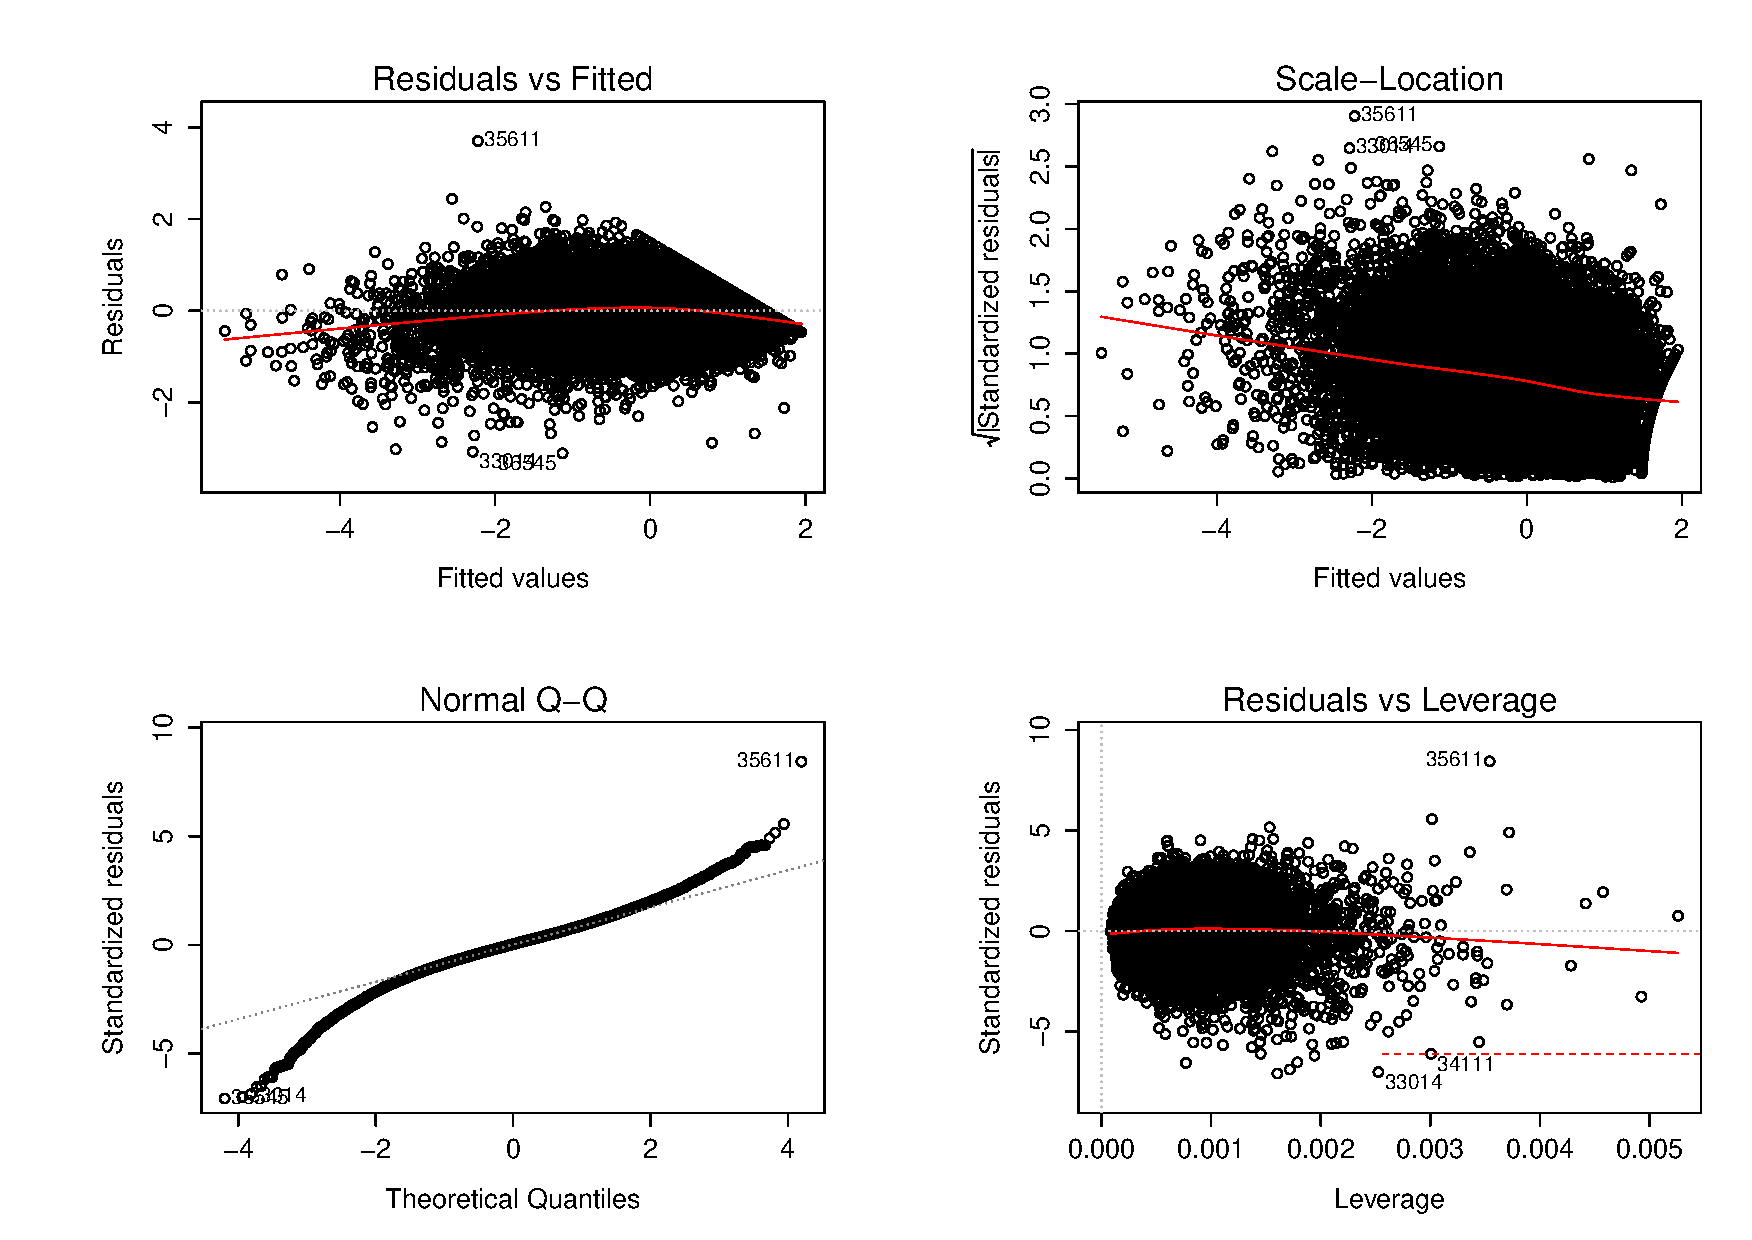
\includegraphics[scale=0.5]{images/ResidualPlots.pdf}~\\		
		\end{center}
		\caption{Residual Plots for Model 3}
		\label{fig:resids}
	\end{figure}
	
Figure \ref{fig:resids} also shows that there are two consistent outlying values, with ID numbers 35611 and 33041. These observations are respectively from Southampton Solent University (10006022): Ocean Sciences and University of Brighton (10000886): Civil Engineering. 

Following visual residual analyses another was conducted for autocorrelation of the residuals. In order to do this the Durbin-Watson test was used, which returned a value of 1.9 ($p < 0.001$), which is very close to the optimal value of 2 \cite{durbin1950testing}. Therefore the model does not suffer from autocorrelation of the residuals. 

Finally, the dataset was searched for influential observations which could have an effect on the final model. Initially leverage was considered to assess which observations exerted the most, using their hat-values. 

The shape of the plot in Figure \ref{fig:LeveragePlot} suggests that there are many more observations with greater leverage in later years, with a sharp increase in the number of observations with higher leverage in 2015, though there is no immediate explanation as to why. It could be related to the fact that in 2015 the restrictions on the availability of NSS data changed, allowing much more to be published than in previous years (as described in Section \ref{limitations}). The five observations with leverage $>$ 0.004 are all from 2015, though with no discernible pattern to unite them aside from the year in which they were sampled. 

\begin{figure}[H]
	\begin{center}
		\includegraphics[scale=0.4]{images/LeveragePlot}~\\		
		\caption{Plot of Hat-Values(/Leverage) for NSS percentage agreement data}
		\label{fig:LeveragePlot}
	\end{center}
\end{figure}


The same can be seen in the Cook's Distance plot in Figure \ref{fig:CooksPlot}, which plots observations against their respective influence. As can be seen there is one observation, highlighted in red, which clearly has a much higher influence than the others. Again it is from 2015, and in general there is a clear increase in the influence from 2015 observations.

\begin{figure}[H]
	\begin{center}
		\includegraphics[scale=0.4]{images/CooksDPlot}~\\		
		\caption{Plot of Cook's Distance Values for NSS percentage agreement data}
		\label{fig:CooksPlot}
	\end{center}
\end{figure}

\section{Year by Year Analysis}
A question that arises when considering the results of the data is whether the important predictors are consistent year-on-year with the ten year analysis. In order to test this, the data were sub-sectioned and standardised by year, then modelled using the final regression model in order to assess the influence of each variable. The results can be seen in Table \ref{table:yearonyear}, which shows the model for each year in order. 

What can be seen when this analysis is carried out is that Q15 is consistently the most important predictor of OS, followed by Q4 then Q1. Often throughout the years Q10 and Q19 also become important, for instance in 2011 these are the only variables with coefficients greater than 0.1, and they switch between as the years go by. However for the most part the three questions already identified are by far the most important year on year, which suggests that their importance is not the result of a trend over the years but a consistent feature of the data throughout the time the NSS has been running. 

\begin{sidewaystable}
[p] \centering \tiny
\caption{Results of Year-By-Year Multiple Regression Models with Sub-setted Data} 
\label{table:yearonyear} 
\begin{tabular}{@{\extracolsep{8pt}}lcccccccccc} 
	\\[-1.8ex]\hline 
	\hline \\[-1.8ex] 
	& \multicolumn{10}{c}{\textit{Model Year:}} \\ 
	\cline{2-11} 
	\\[-1.8ex] & \multicolumn{10}{c}{OS} \\ 
	\\[-1.8ex] & 2006 & 2007 & 2008 & 2009 & 2010 & 2011 & 2012 & 2013 & 2014 & 2015\\ 
	\hline \\[-1.8ex] 
	Q1 & 0.209$^{***}$ & 0.211$^{***}$ & 0.151$^{***}$ & 0.192$^{***}$ & 0.198$^{***}$ & 0.179$^{***}$ & 0.170$^{***}$ & 0.172$^{***}$ & 0.157$^{***}$ & 0.151$^{***}$ \\ 
	& (0.016) & (0.015) & (0.014) & (0.014) & (0.013) & (0.012) & (0.012) & (0.009) & (0.013) & (0.011) \\ 
	& & & & & & & & & & \\ 
	Q2 & 0.038$^{**}$ & 0.015 & 0.043$^{***}$ & 0.015 & 0.035$^{**}$ & 0.047$^{***}$ & 0.059$^{***}$ & 0.046$^{***}$ & 0.080$^{***}$ & 0.057$^{***}$ \\ 
	& (0.017) & (0.016) & (0.015) & (0.015) & (0.014) & (0.014) & (0.014) & (0.010) & (0.014) & (0.012) \\ 
	& & & & & & & & & & \\ 
	Q3 & 0.035$^{**}$ & 0.009 & 0.058$^{***}$ & 0.021 & 0.002 & 0.014 & 0.004 & 0.042$^{***}$ & 0.046$^{***}$ & 0.039$^{***}$ \\ 
	& (0.017) & (0.015) & (0.014) & (0.014) & (0.013) & (0.013) & (0.013) & (0.009) & (0.012) & (0.011) \\ 
	& & & & & & & & & & \\ 
	Q4 & 0.193$^{***}$ & 0.202$^{***}$ & 0.195$^{***}$ & 0.192$^{***}$ & 0.227$^{***}$ & 0.244$^{***}$ & 0.224$^{***}$ & 0.209$^{***}$ & 0.195$^{***}$ & 0.174$^{***}$ \\ 
	& (0.015) & (0.014) & (0.012) & (0.013) & (0.012) & (0.012) & (0.012) & (0.008) & (0.011) & (0.010) \\ 
	& & & & & & & & & & \\ 
	Q5 & $-$0.022 & $-$0.024$^{**}$ & 0.008 & $-$0.0003 & $-$0.002 & $-$0.007 & 0.015 & $-$0.030$^{***}$ & $-$0.008 & 0.008 \\ 
	& (0.013) & (0.012) & (0.011) & (0.011) & (0.010) & (0.010) & (0.010) & (0.007) & (0.010) & (0.010) \\ 
	& & & & & & & & & & \\ 
	Q6 & 0.074$^{***}$ & 0.080$^{***}$ & 0.084$^{***}$ & 0.054$^{***}$ & 0.061$^{***}$ & 0.043$^{***}$ & 0.026$^{**}$ & 0.082$^{***}$ & 0.045$^{***}$ & 0.037$^{***}$ \\ 
	& (0.014) & (0.013) & (0.011) & (0.011) & (0.011) & (0.010) & (0.011) & (0.007) & (0.010) & (0.010) \\ 
	& & & & & & & & & & \\ 
	Q7 & $-$0.023 & $-$0.003 & $-$0.015 & 0.016 & $-$0.016 & $-$0.006 & $-$0.015 & $-$0.005 & 0.010 & 0.005 \\ 
	& (0.014) & (0.014) & (0.012) & (0.012) & (0.011) & (0.011) & (0.011) & (0.008) & (0.010) & (0.010) \\ 
	& & & & & & & & & & \\ 
	Q8 & 0.037$^{*}$ & 0.010 & $-$0.003 & $-$0.010 & $-$0.007 & $-$0.024$^{*}$ & $-$0.003 & $-$0.013 & $-$0.038$^{***}$ & $-$0.027$^{**}$ \\ 
	& (0.019) & (0.017) & (0.015) & (0.015) & (0.014) & (0.014) & (0.014) & (0.010) & (0.014) & (0.012) \\ 
	& & & & & & & & & & \\ 
	Q9 & $-$0.024 & $-$0.006 & $-$0.011 & $-$0.019 & $-$0.012 & 0.008 & $-$0.005 & $-$0.018$^{*}$ & $-$0.011 & $-$0.001 \\ 
	& (0.020) & (0.017) & (0.016) & (0.015) & (0.014) & (0.014) & (0.014) & (0.010) & (0.014) & (0.013) \\ 
	& & & & & & & & & & \\ 
	Q10 & 0.088$^{***}$ & 0.086$^{***}$ & 0.074$^{***}$ & 0.088$^{***}$ & 0.119$^{***}$ & 0.115$^{***}$ & 0.085$^{***}$ & 0.094$^{***}$ & 0.110$^{***}$ & 0.127$^{***}$ \\ 
	& (0.018) & (0.016) & (0.015) & (0.014) & (0.014) & (0.013) & (0.014) & (0.010) & (0.013) & (0.012) \\ 
	& & & & & & & & & & \\ 
	Q11 & 0.066$^{***}$ & 0.062$^{***}$ & 0.043$^{***}$ & 0.058$^{***}$ & 0.012 & 0.011 & 0.022$^{**}$ & 0.023$^{***}$ & 0.038$^{***}$ & 0.043$^{***}$ \\ 
	& (0.016) & (0.015) & (0.013) & (0.012) & (0.011) & (0.011) & (0.011) & (0.008) & (0.010) & (0.009) \\ 
	& & & & & & & & & & \\ 
	Q12 & $-$0.011 & 0.018 & 0.00000 & 0.030$^{**}$ & 0.008 & 0.001 & 0.019 & 0.007 & $-$0.009 & 0.004 \\ 
	& (0.016) & (0.015) & (0.013) & (0.013) & (0.013) & (0.012) & (0.013) & (0.009) & (0.012) & (0.011) \\ 
	& & & & & & & & & & \\ 
	Q13 & $-$0.057$^{***}$ & $-$0.020 & $-$0.020$^{*}$ & $-$0.004 & $-$0.010 & $-$0.022$^{**}$ & $-$0.038$^{***}$ & $-$0.040$^{***}$ & $-$0.032$^{***}$ & $-$0.032$^{***}$ \\ 
	& (0.013) & (0.012) & (0.011) & (0.011) & (0.010) & (0.010) & (0.010) & (0.007) & (0.009) & (0.009) \\ 
	& & & & & & & & & & \\ 
	Q14 & 0.016 & $-$0.010 & $-$0.033$^{**}$ & $-$0.044$^{***}$ & $-$0.013 & 0.022 & $-$0.014 & $-$0.002 & $-$0.013 & 0.021$^{*}$ \\ 
	& (0.020) & (0.018) & (0.016) & (0.016) & (0.015) & (0.014) & (0.015) & (0.010) & (0.014) & (0.012) \\ 
	& & & & & & & & & & \\ 
	Q15 & 0.414$^{***}$ & 0.378$^{***}$ & 0.420$^{***}$ & 0.393$^{***}$ & 0.360$^{***}$ & 0.337$^{***}$ & 0.379$^{***}$ & 0.369$^{***}$ & 0.364$^{***}$ & 0.328$^{***}$ \\ 
	& (0.022) & (0.020) & (0.018) & (0.018) & (0.017) & (0.016) & (0.016) & (0.011) & (0.015) & (0.013) \\ 
	& & & & & & & & & & \\ 
	Q16 & 0.053$^{***}$ & 0.051$^{***}$ & 0.023$^{**}$ & 0.043$^{***}$ & 0.032$^{***}$ & 0.050$^{***}$ & 0.053$^{***}$ & 0.049$^{***}$ & 0.053$^{***}$ & 0.048$^{***}$ \\ 
	& (0.013) & (0.012) & (0.011) & (0.011) & (0.010) & (0.009) & (0.010) & (0.007) & (0.010) & (0.009) \\ 
	& & & & & & & & & & \\ 
	Q17 & 0.011 & 0.022$^{*}$ & 0.016 & 0.007 & 0.006 & 0.003 & $-$0.020$^{*}$ & $-$0.006 & $-$0.024$^{**}$ & $-$0.0004 \\ 
	& (0.015) & (0.013) & (0.011) & (0.011) & (0.011) & (0.010) & (0.011) & (0.007) & (0.010) & (0.010) \\ 
	& & & & & & & & & & \\ 
	Q18 & $-$0.035$^{**}$ & $-$0.034$^{***}$ & $-$0.002 & $-$0.012 & 0.002 & $-$0.021$^{**}$ & 0.0002 & $-$0.032$^{***}$ & $-$0.007 & $-$0.012 \\ 
	& (0.014) & (0.013) & (0.012) & (0.012) & (0.011) & (0.011) & (0.011) & (0.007) & (0.011) & (0.010) \\ 
	& & & & & & & & & & \\ 
	Q19 & 0.084$^{***}$ & 0.077$^{***}$ & 0.088$^{***}$ & 0.090$^{***}$ & 0.092$^{***}$ & 0.113$^{***}$ & 0.109$^{***}$ & 0.088$^{***}$ & 0.100$^{***}$ & 0.089$^{***}$ \\ 
	& (0.016) & (0.015) & (0.013) & (0.013) & (0.012) & (0.012) & (0.013) & (0.009) & (0.012) & (0.011) \\ 
	& & & & & & & & & & \\ 
	Q21 & 0.065$^{***}$ & 0.089$^{***}$ & 0.062$^{***}$ & 0.078$^{***}$ & 0.074$^{***}$ & 0.071$^{***}$ & 0.092$^{***}$ & 0.104$^{***}$ & 0.086$^{***}$ & 0.081$^{***}$ \\ 
	& (0.016) & (0.015) & (0.013) & (0.013) & (0.012) & (0.012) & (0.013) & (0.009) & (0.012) & (0.011) \\ 
	& & & & & & & & & & \\ 
	Constant & 0.000 & $-$0.000 & 0.000 & 0.000 & 0.000 & 0.000 & 0.000 & 0.000 & 0.000 & $-$0.000 \\ 
	& (0.010) & (0.009) & (0.008) & (0.008) & (0.007) & (0.007) & (0.007) & (0.005) & (0.007) & (0.007) \\ 
	& & & & & & & & & & \\ 
	\hline 
	\hline \\[-1.8ex] 
	\textit{Note:}  & \multicolumn{10}{r}{$^{*}$p$<$0.1; $^{**}$p$<$0.05;  $^{***}$p$<$0.01} \\ 
\end{tabular} 
\end{sidewaystable}

\section{Interpretation of Results}
The regression conducted has given some indication as to what the underlying causes of student satisfaction are. Given that the regression analysis and the correlation matrix both suggested the same conclusion it can be inferred that 
\begin{quote}
	Q15. The course is well organised and running smoothly\\
	Q4. The course is intellectually stimulating\\
	Q1. Staff are good at explaining things\\
\end{quote}
are the biggest predictors of Q22, Overall Satisfaction. The fact that there are two questions from the `Teaching on my course' thematic area is also suggestive that satisfactory teaching is an area that is most likely to benefit a department or institution. The importance of teaching as a factor in student satisfaction has been suggested previously \cite{ginns2007students}, and is consistent with the findings by HEFCE in their review of the NSS \cite{HEFCEreport2014}. However there are very few results that suggest the organisation of a course is of great importance to students.

The model obtained using the forward-selection method retained 20 of the 21 independent variables, disposing only of Q20 (`My communication skills have improved'). This is consistent with views that student satisfaction is multi-faceted, and so would logically be related to all variables that have some consequence in interpreting it. However, this could also be a reflection of the fact that the NSS is a `well-designed' survey and all questions are related to the outcome question. It is possible that the regression modelling used does not acknowledge key features of the data, such as its hierarchical structure, and that doing so may result in a reduced model.

It can be concluded that the regression modelling of the NSS was successful, however due to the nature of the data it would be beneficial to use more sophisticated modelling techniques. 
\newpage

\chapter{Multilevel Modelling}
When working with hierarchical data it is important to incorporate the structure of the data into the modelling process, and so to more accurately represent the data multilevel modelling was employed following the regression modelling stage. The following chapter describes the development process that led to the final model, and explores the validity and implications of this model. 

\section{Model Development}
\subsection{Initial Model}

\begin{figure}
	\centering
	\includegraphics[width=1\linewidth]{images/MLMmodels}
	\caption{The model building process described diagrammatically. Dotted lines represent models tested for their significance against models on the left of the diagram.}
	\label{fig:MLMmodels}
\end{figure}

The first stage in implementing the model, as described in Section \ref{methodMLM}, was to test the suitability of the nesting structure described in Figure \ref{fig:MLMStructure}, that is testing the null hypothesis that there are no random effects described by the hierarchical structure. In order to do this an initial model (Model 1) was constructed with only a fixed intercept and random intercepts for Institution and Subject within Institution. This is described algebraically as: 
\[OS_{ijk} = \beta_{0} + V_{k} + u_{jk} + e_{ijk}, \]
\[V_{k} \sim N(0, \sigma^{2}_v), u_{jk} \sim N(0, \sigma^{2}_u), e_{ijk} \sim N(0, \sigma^{2}_e)\]

where
$\beta_{0}$ is the mean response across all institutions, 
$V_{k}$ the effect of institution $k$,
$u_{jk}$ the effect of subject $j$ within institution $k$, and
$e_{ijk}$ the residual error term.

\newpage
Model 2 was then constructed, also with a fixed intercept but instead with only random intercepts for Institution. This is described algebraically as: 
\[OS_{i k} = \beta_{0} + u_{ k} + e_{i k} \]
\[u_{i} \sim N(0, \sigma^{2}_u), e_{i k} \sim N(0, \sigma^{2}_e) \]

where
$\beta_{0} =$ mean response across all institutions,
$u_{ k} =$ effect of institution  $k$, and
$e_{i k} =$ residual error term.

Using the R language specification for multilevel models (from the package LME4 \cite{R_lme4}) is often a clearer way to represent the specifications of these models as it uses Wilkinson and Rogers' original notation for models for analysis of variance, combined with computer programming notation \cite{wilkinson1973symbolic}. Here we have: 
{\footnotesize
\begin{lstlisting}[backgroundcolor = \color{light-gray}, language=R, escapechar=±]
 > Model1 <- OS ±$\sim$± 1 + (1|Inst/Subject)
 > Model2 <- OS ±$\sim$± 1 + (1|Inst)
\end{lstlisting}
}
where OS $\sim$ indicates that OS is the dependent variable, the 1 represents the fixed intercept, and the terms in brackets represent random intercepts for Institution in Model 2, as well as Subject within Institution for Model 1. 

Comparing Model 1 and Model 2 using a chi-squared test on their log-likelihood ratio revealed that the nesting structure is highly significant ($p < 0.001$) and so Model 1 with the nesting structure for the random intercepts should be retained.

The next stage was to test whether adding the fixed effects made a significant difference to the model. In this instance the fixed effects were the 21 independent variables, which were added to create Model 3, alongside the random intercepts for Institution and Subject within Institution. Once again using a chi-squared test to compare Model 1 and Model 3 showed that the fixed effects were highly significant ($p < 0.001$) and should remain in the model; additionally it can be observed in Figure \ref{fig:MLMModelResults} that the \ac{BIC} had reduced, which is a sign that the model is better fit for the data. Since there are no independent variables at Levels 2 or 3 this was the end of the manual model building process. 

{\footnotesize
\begin{lstlisting}[backgroundcolor = \color{light-gray}, language=R, escapechar=±]
 > Model3 <- OS ±$\sim$± Q1 + Q2 + Q3 + Q4 + Q5 + Q6 + Q7 + Q8 + Q9 + Q10 + Q11
  + Q12 + Q13 + Q14 + Q15 + Q16 + Q17 + Q18 + Q19 + Q20 + Q21 
  + (1|Inst/Subject)
\end{lstlisting}
}

The next stage was to employ the automatic model selection function in R, which would backward-fit the fixed effects and later forward fit the random effects, specified in an array as a function argument. The function allows the user to choose a certain number of other arguments so that the statistic used to test the model was the $p$-value, with a threshold of 0.05, and the method used to fit it was the BIC, with a minimum change threshold of 5 since this is less likely to result in Type I errors in the model than using $p$-values. It was also specified in the arguments for the model that it should remove any random effect for which its variable is not also present in the fixed effects structure. 

In the first instance this caused a number of issues due to the size and complexity of both the model and the dataset. The runtime for the function exceeded a reasonable level (12+ hours) and so a different approach was attempted. This time the fixed effects were backward-fitted, and then only those variables present in the fixed effects were forward-fitted as random intercepts and slopes. 
In the first stage the model retained 14 of the 21 independent variables, resulting in the following model as specified using LMER, 

{\footnotesize
\begin{lstlisting}[backgroundcolor = \color{light-gray}, language=R, escapechar=±]
 > Model4 <- OS ±$\sim$± Q1 + Q2 + Q3 + Q4 + Q6 + Q7 + Q8 + Q10 + Q11 
  + Q14 + Q15 + Q17 + Q19 + Q21 + (1|Inst/Subject)
\end{lstlisting}
}
where the final term specifies inclusion of random intercepts for Institution and Subject within Institution, rendering this an intercept-only model. In the next stage the model was tested for the inclusion of all random effects related to the fixed effects, where it would then become a mixed model.

\subsection{Introducing Random Effects}
When attempting to forward-fit the random effects, with 14 of them instead of 21 to match the fixed effects, the model ran for over 96 hours without completing, however all the random effects that were processed in that time were added to the model. As a result it was decided to keep all the random effects related to the fixed effects in Model 4, in order to create Model 5. Another strategy could have been to fit a model where random slopes and intercepts are assumed to be independent and their correlation is zero, a commonly used option to reduce the complexity of multilevel models \cite{bates2014fitting}. However the drawback is that the model becomes more sensitive to shifts in the predictor variable, and it was preferred to avoid this approach if possible. 

\newpage
{\footnotesize
\begin{lstlisting}[backgroundcolor = \color{light-gray}, language=R, escapechar=±]
 > Model5 <- OS ±$\sim$± Q1 + Q2 + Q3 + Q4 + Q6 + Q7 + Q8 + Q10 + Q11 + Q14 + Q15
  + Q17 + Q19 + Q21 + (1|Inst/Subject) + (Q1|Inst/Subject)
  + (Q2|Inst/Subject) + (Q3|Inst/Subject) + (Q4|Inst/Subject) 
  + (Q6|Inst/Subject) + (Q7|Inst/Subject) + (Q8|Inst/Subject)
  + (Q10|Inst/Subject) + (Q11|Inst/Subject) + (Q14|Inst/Subject)
  + (Q15|Inst/Subject) + (Q17|Inst/Subject) + (Q19|Inst/Subject)
  + (Q20|Inst/Subject)
\end{lstlisting}
}
A chi-squared test on the log-likelihood values revealed that Model 5 was an improvement upon Model 4, with a significance of $p<$0.001. At each stage of model development the new model has been seen to be a significant improvement on the last, and for each model the BIC had improved. Model 5 represents a point at which any further developments in terms of adding fixed effects does not weigh up against the computation exertion they elicit, therefore it is the final model in this stage. 

\subsection{Adding Interaction Terms}
Whilst there is no way to further improve the model by adding random effects or otherwise, one development not yet considered is the addition of interaction effects to the model. While correlations regard the relationship between two variables, an interaction effect considers the relationship between two variables with regard to their joint effect on a third.  	

The choice of which interactions to include in the model depends on the design of the study, and reading further into the meaning behind the variables. Some studies are designed exclusively to examine interaction effects but the NSS is not one of these, and so it more appropriate to consider which variables may interact, and then to test what happens when these effects are introduced to the model. 

Considering the list of questions in the NSS, there are some variables which appear likely to interact with each other, with a short explanation as to why:

\begin{tabular}{ll}
\textbf{Q2*Q3:} & Staff making the course interesting by being enthusiastic about teaching,\\
Q5*Q6: & Assessment being fair requires criteria for marking to be clear in advance, \\
\textbf{Q14*Q15:} & Good communication on a course requires good organisation,\\
Q16*Q17: & Good library services require good IT services.
\end{tabular}\\


Given that not all of these variables are still included in the model those still available to be added are highlighted in bold above. Due to the computational complexity of processing the model, a model (Model 6) was first run without the random effects to see whether adding the interaction effects to the fixed effects was significant and reduced the BIC. It can be seen in Figure \ref{fig:MLMmodels} that Model 6 is essentially an extension of Model 4. The specification for Model 6 represents the interactions using *. 

{\footnotesize
\begin{lstlisting}[backgroundcolor = \color{light-gray}, language=R, escapechar=±]
> Model6 <- OS ±$\sim$± Q1 + Q2*Q3 + Q4 + Q6 + Q7 + Q8 + Q10 + Q11 + Q14*Q15
 + Q17 + Q19 + Q21 + (1|Inst/Subject)
\end{lstlisting}
}

It was found that there was a significant improvement between Models 4 and 6 and so it was worth using computational resources to process a model with interaction terms and random effects. Given this successful improvement, Model 7 was created. 

{\footnotesize 
\begin{lstlisting}[backgroundcolor = \color{light-gray}, language=R, escapechar=±]
 > Model7 <- OS ±$\sim$± Q1 + Q2*Q3 + Q4 + Q6 + Q7 + Q8 + Q10 + Q11 + Q14*Q15
  + Q17 + Q19 + Q21 + (1|Inst/Subject) + (Q1|Inst/Subject)
  + (Q2|Inst/Subject) + (Q3|Inst/Subject) + (Q4|Inst/Subject) 
  + (Q6|Inst/Subject) + (Q7|Inst/Subject) + (Q8|Inst/Subject)
  + (Q10|Inst/Subject) + (Q11|Inst/Subject) + (Q14|Inst/Subject)
  + (Q15|Inst/Subject) + (Q17|Inst/Subject) + (Q19|Inst/Subject)
  + (Q20|Inst/Subject)
\end{lstlisting}
}

It is noted that the interaction effects were not also included for the random effects as this approach caused several computational issues. As a result the interactions are only between the fixed effects and the random effects have remained additive. Model 7 was once again significantly more successful than its predecessor, Model 5 and thus it was decided that Model 7 was the final model resulting from this process, as can be observed in Figure \ref{fig:MLMModelResults}. 

\begin{figure}
\centering
\includegraphics[width=1\linewidth]{images/MLMModelResults}
\caption{Development of the Multilevel Model Building Process, measured using BIC}
\label{fig:MLMModelResults}
\end{figure}

The estimates for the parameters of Model 7 are displayed in Tables \ref{Table:RandomEffectsM7} and \ref{Table:FixedEffectsM7}, where Figure \ref{fig:RaneffPredict} shows the 95\% prediction intervals on the random effects in Model 7 for both Institution and also Subject within Institution versus the quantiles of the standard normal distribution. Where there are a large number of estimated random effects, as there are here, these plots can assist with interpreting patterns in the estimated effects. 


\begin{table}
	\centering
\caption{Random Effects Estimates for Model 7}
\label{Table:RandomEffectsM7}
\begin{tabular}{@{\extracolsep{5pt}}lrrrr}
\hline \hline
 & & & & \\
& \multicolumn{2}{c}{\textit{Subject in Institution}} & \multicolumn{2}{c}{\textit{Institution}} \\
\cline{2-5}
 & & & &\\
\textit{Random Effect} & Variance & Std.Dev. & Variance & Std.Dev. \\[0.1cm]
\hline
(Intercept) & 8.018e-04  & 0.028316          	&7.432e-04 &0.027261 \\      
Q1         & 1.119e-02  & 0.105787 		      &1.314e-03 &0.036255 \\[0.3cm]

(Intercept) & 2.841e-03  & 0.053298            &1.794e-03 &0.042358 \\     
Q2          & 9.361e-03  & 0.096755      &8.281e-04 &0.028778 \\[0.3cm]

(Intercept) & 6.655e-04  & 0.025798            &3.458e-04 &0.018595 \\      
Q3          & 9.838e-03  & 0.099185      &6.180e-04 &0.024859 \\[0.3cm]

(Intercept) & 6.545e-03  & 0.080900          	&2.481e-03 &0.049809 \\   
Q4         & 1.499e-02  & 0.122420     	&9.531e-04 &0.030872 \\[0.3cm]

(Intercept) & 1.746e-03  & 0.041789            &1.172e-03 &0.034238 \\
Q6         & 8.907e-03  & 0.094378    	&2.951e-04 &0.017180 \\[0.3cm]

(Intercept) & 1.003e-03  & 0.031674          	&3.644e-04 &0.019090 \\     
Q7          & 5.940e-03  & 0.077068      &6.062e-04 &0.024621 \\[0.3cm]

(Intercept) & 0.000e+00  & 0.000000            &1.524e-04 &0.012345 \\   
Q8          & 2.504e-03  & 0.050035        &2.873e-04 &0.016951 \\[0.3cm]

(Intercept) & 7.300e-04  & 0.027018            &1.851e-03 &0.043020 \\ 
Q10         & 5.164e-03  & 0.071860      &9.191e-04 &0.030317 \\[0.3cm]

(Intercept) & 1.826e-03  & 0.042736          	&2.348e-04 &0.015323 \\
Q11         & 1.129e-02  & 0.106254      &5.643e-04 &0.023755 \\[0.3cm]

(Intercept) & 1.514e-03  & 0.038908          	&3.292e-04 &0.018144 \\ 
Q14         & 1.215e-02  & 0.110246      &1.456e-03 &0.038158 \\[0.3cm]

(Intercept)& 6.831e-03  & 0.082652          	&2.908e-03 &0.053923 \\  
Q15         & 1.261e-02  & 0.112280      &1.220e-03 &0.034933 \\[0.3cm]

(Intercept) & 6.010e-05  & 0.007752          	&1.651e-06 &0.001285 \\ 
Q17        & 8.114e-03  & 0.090075    	&3.891e-04 &0.019724 \\[0.3cm]

(Intercept) & 1.758e-03  & 0.041927 		  	&2.910e-03 & 0.053946 \\
Q19         & 7.916e-03  & 0.088971  	&1.189e-03 & 0.034478 \\[0.3cm]

(Intercept) & 1.253e-03 & 0.035398  			& 1.656e-03 & 0.040692 \\ 
Q21         & 6.653e-03 & 0.081568       &8.600e-04 & 0.029325  \\[0.3cm]

Intercept   & 0.000e+00  & 0.000000          	&0.000e+00 &0.000000 \\[0.3cm]     
   
Residual &				& 			 			& 8.897e-02 & 0.298272 \\[0.3cm]
\hline \hline
\end{tabular}     
\end{table}



\begin{table}
	\centering
	\caption{Fixed Effects Estimates for Model 7}
	\label{Table:FixedEffectsM7}
\begin{tabular}{@{\extracolsep{5pt}}lrrr}
	\hline \hline
	& & &  \\
	\textit{Fixed Effect}	&	Estimate	& Std. Error & t value \\[0.3cm]
	\hline
	(Intercept) & -0.0006964 & 0.0101972  & -0.07 \\[0.2cm]
	Q1          & 0.1588488  &0.0053577   &29.65\\[0.2cm]
	Q2          & 0.0781380  &0.0053079   &14.72\\[0.2cm]
	Q3          & 0.0279086  &0.0049184   & 5.67\\[0.2cm]
	Q4          & 0.1854301  &0.0051798   &35.80\\[0.2cm]
	Q6          & 0.0687747  &0.0039030   &17.62\\[0.2cm]
	Q7          &-0.0173524  &0.0044511   &-3.90\\[0.2cm]
	Q8          &-0.0211510  &0.0043752   &-4.83\\[0.2cm]
	Q10         & 0.1058575  &0.0049537   &21.37\\[0.2cm]
	Q11         & 0.0191679  &0.0045214   & 4.24\\[0.2cm]
	Q14         &-0.0280838  &0.0057095   &-4.92\\[0.2cm]
	Q15         & 0.3213007  &0.0061082   &52.60\\[0.2cm]
	Q17         & 0.0166124  &0.0034327   & 4.84\\[0.2cm]
	Q19         & 0.0910560  &0.0050502   &18.03\\[0.2cm]
	Q21         & 0.0669559  &0.0047334   &14.15\\[0.2cm]
	Q2:Q3       &-0.0166004  &0.0023582   &-7.04\\[0.2cm]
	Q14:Q15     &-0.0351616  &0.0024652   &-14.26\\[0.2cm]
	\hline \hline
\end{tabular}
\end{table}

\begin{table}
	\centering
	\caption{Model Fit Tests for Model 7}
	\begin{tabular}{@{\extracolsep{5pt}}lllll}
		\hline \hline
		AIC & BIC & logLik & deviance & df.resid \\[0.2cm]
		\hline
		36855.5 & 37741.5 & -18323.7 & 36647.5 & 36926 \\[0.2cm]
		\hline \hline
	\end{tabular}
\end{table}

\begin{figure}[h]
	\centering
		\subfigure[Institution]{\includegraphics[width=0.49\textwidth]{images/RaneffPredictInst}}
		\subfigure[Subject within Institition]{\includegraphics[width=0.49\textwidth]{images/RaneffPredictSubjInst}}
		\caption{Prediction Intervals for Random Effects in Model 7}
		\label{fig:RaneffPredict}
\end{figure}

One of the benefits of multilevel modelling is the ability to assess the \ac{ICC}. The ICC is an informative measure of how correlated a group is with relation to other groups nested under the same structure, where for each level of nesting an ICC can be specified as a function of the variance components so that here two ICC values can be calculated, the institution-level ICC and the subject-level ICC. Given that the primary interest is in these two singular values it is not appropriate to use the variance components from Model 7 to calculate them as these would give the ICC individually for each question, which is unnecessary. As a result, the ICC can be computed from the results of Model 6, where random effects only varied over the intercept, but the model still followed the same fixed effects structure as in Model 7. 

Taking the variance of random effects associated with institutions as $\sigma^{2}_i$, and the variance of random effects associated with subjects nested in institutions as $\sigma^{2}_s$ we obtain the following equations for ICC: 
\[ICC_{institution} = \frac{\sigma^{2}_i}{\sigma^{2}_i + \sigma^{2}_s + \sigma^{2}} \]
\[ICC_{subject} = \frac{\sigma^{2}_i + \sigma^{2}_s}{\sigma^{2}_i + \sigma^{2}_s + \sigma^{2}} \]

For Model 6 the variances of the random effects were $\sigma^{2}_i = 0.01272$, $\sigma^{2}_s = 0.03158$ and residual variance, $\sigma^{2} = 0.15598$, which gives the corresponding ICCs:
\[ICC_{institution} = \frac{0.01272}{0.01272 + 0.03158 + 0.15598} = 0.06 \] 
\[ICC_{subject} = \frac{0.01272 + 0.03158}{0.01272 + 0.03158 + 0.15598} = 0.22\]

Therefore there is large variation within institutions and thus small variation between them which leads to a modest ICC, whereas for subjects within institutions there is slightly higher ICC, as there is less variability within subjects within institutions, and thus more variability between them. 
 

\section{Validation}
Validating the final model in the same way as in Section \ref{regmodelvalidation} using CV is more difficult for multilevel models than for regression models due to ambiguity in how to train and test the data whilst considering the hierarchical structure. Additionally, the random effects can disrupt the loss functions estimated during the CV process which results in poorly estimated prediction error; this is reiterated in the statistical documentation for R which states that there is no option for computing standard errors of predictions because it is difficult to define an efficient method that incorporates uncertainty in the variance parameters \cite{R_lme4}. Due to these issues, as discussed by Wang and Gelman \cite{wang2014difficulty}, there is need for due caution when using this technique on structured models, and even when it is used there may be a surprisingly small improvement between a regular multiple regression approach and a multilevel one, which is not true to the actual success of the model.

It has been shown that considering the \ac{AIC} is equivalent to leave-one-out CV \cite{fang2011asymptotic, stone1977asymptotic}, however this usage is more appropriate for model selection that prediction error estimates. 

As a result in this instance it was deemed inappropriate to attempt model validation, and instead to concentrate on the diagnostic test results of the model to ensure its accuracy. 


\newpage
\section{Diagnostic Tests} \label{MLMdiagnostics}
Similarly to the case of regression analysis it is necessary to check several assumptions in the model, and in order to so the residual plots will be examined. There would usually be scope to explore further with formal testing and influence measures such as Cook's distance; however this is not possible with a model of this complexity. Despite it being possible to residual analysis there is very little advice or information in the literature about conducting diagnostic tests for highly complex models with large datasets and is something that needs to be developed and researched in order to be able to validate these models properly. 

When conducting the residual analysis it is noted that this model is not created in order to make highly accurate predictions of OS, its purpose being much more general in giving an idea of which variables may be more important than others. With this in mind it is not necessary for the model to perfectly meet the assumptions of a linear multilevel model, though it is necessary to be aware of any violations. 

\begin{figure}[H]
	\centering
	\includegraphics[width=0.95\linewidth]{images/SresidvfittedMLM}
	\caption{Standardized Residuals at Level 1 of Model 7}
	\label{fig:SresidvfittedMLM}
\end{figure}
\begin{figure}[H]
	\centering
	\includegraphics[width=0.95\linewidth]{images/qqplotmodel7}
	\caption{Normal QQ Plot for Standardized Residuals at Level 1 of Model 7}
	\label{fig:qqplotmodel7}
\end{figure}


To begin with a standardized residual and a normal Q-Q plot were created at the first level of the model where the fixed effects are specified and can be seen in Figures \ref{fig:SresidvfittedMLM} and \ref{fig:qqplotmodel7}; the residuals for the random effects at Levels 2 and 3 are examined later. These diagrams clearly reveal an issue with heteroscedasticity in the model, identified by the distinct funnel shape. 

In terms of normality it can be seen in Figure \ref{fig:qqplotmodel7} that at Level 1 of the model there is a satisfactory level of normality in the residuals, given the fairly linear trend created by the points on the plot. The normal Q-Q plot also reveals three outliers, two at the left-hand of the tail and one at the right. The right-hand outlier is for Accounting at Anglia Ruskin University and the two left-hand outliers are Sociology at the University of Bristol and Theology and Religious Studies at University of Sheffield. This appears to be because the two left-hand courses performed much worse than would be predicted under a normal curve, and the right-hand observation performed much better. 

When there are random effects in addition to the standard error term, as there are here, we can use normal probability plots of the estimated random effects to test for normality in the random effects; in order to do this the \ac{EBLUP} are plotted and examined \cite{Lawson201412}. 

\begin{figure}[h]
	\centering
		\subfigure{\includegraphics[width = 0.49\textwidth]{images/EBLUPinst.pdf}} 
		\subfigure{\includegraphics[width = 0.49\textwidth]{images/EBLUPsubjinst.pdf}}
		\caption{Normal QQ Plots for EBLUP scores}
		\label{fig:EBLUPplots}
\end{figure}
		
		
As can be seen in Figure \ref{fig:EBLUPplots} there is non-normality present in the EBLUP distribution which is evidence that the residuals in the random effects vary hugely, and that there are many institutions that perform much better, and much worse than those considered `standard'. However, often there is more value in using the EBLUP plots to consider outliers than normality, since their distribution does not necessarily reflect the true distribution of the random effects \cite{LinearMMs}. Here it can be seen that in each of the two plots there are two distinct outliers at the edge of the tail on each. In Figure \ref{fig:EBLUPplots}(a) the two outlying institutions are London Metropolitan University and the University of Kent, and in Figure \ref{fig:EBLUPplots}(b) the outlying subjects are Imaginative Writing at Sheffield Hallam University and Theology and Religious Studies at Oxford Brookes. These outliers do not correspond to any other outliers encountered at other points in the analysis and do not appear to pose a significant threat to the model. 

\newpage
\section{Interpretation of Results}
It is clear that using a multilevel model to interpret the hierarchical structure of the data available was an appropriate decision and allowed for more detailed and representative modelling than previously in the multiple regression modelling. The most successful model, when measured by the BIC, was that which included the interactions between variables for the those chosen as well as random intercepts and slopes.
There are several important observations from this model, and these include which variables have been discarded from the model and which were kept, what the coefficients of the fixed effects were and the added value from the interaction effects included, as well as minor interpretations of the random effects since they are not of primary interest.  

Firstly, considering the variables discarded during the modelling process gives an indication of which were important and which were not, namely those discarded were:\\
Q5 ``The criteria used in marking have been made clear in advance'',\\ 
Q9 ``Feedback on my work has helped me to clarify things I didn't understand'', \\
Q12 ``Good advice was available when I needed to make study choices'',\\ 
Q13 ``The timetable worked efficiently as far as my activities were concerned'',\\ 
Q16 ``The library resources and services are good enough for my needs'', \\
Q18 ``I have always been able to access specialised equipment, facilities and rooms when needed'', and
Q20 ``My communication skills have improved''.\\ 
These questions came from a range of different thematic areas (see Table \ref{table:NSSquestions}) with at least one removed from each thematic area apart from the first with relation to Teaching, yet no thematic areas which have had all questions removed. This suggests that all the questions from the Teaching area are important, and additionally that there is at least one question from each thematic area which is also worth considering.

For those variables which were retained in the model the fixed effects estimates show that some variables have considerably more influence than others. Primarily Q15 stands out as the variable with the highest influence on the model with an estimate of 0.32, the next highest being Q4 with 0.19. In fact, when considering all the fixed effects estimates as percentages, using their absolute values, the coefficient for Q15 makes up just over 25\% of all the estimate values, which is weighty given there are 14 values in total. In comparison the thematic area of Teaching resembles around 37\% with all four of its questions which would suggest that while it is still highly important, Q15 is more representative as a single question. 

Another feature to consider is the interaction effects which had not previously been included in the regression modelling process. As can be observed in Figure \ref{fig:MLMModelResults} the inclusion of the interactions between Q2 and Q3, and Q14 and Q15 caused a significant reduction in the BIC of over 3800 between Models 4 and 6, and a reduction of over 400 between Models 5 and 7. What is interesting when observing the model results is the similarity in the BIC between Model 5 and Model 6, where model 5 includes all the random slopes and intercepts and Model 6 includes only random intercepts but also the interactions. It seems to suggest that the interaction effects improved the model almost as much as the random slopes did, but with significantly less run-time needed. This may be something to consider for attempts to model the data in the future. 

The last aspect of the multilevel model to discuss is the meaning of the random effects structure and what it reveals about the data. It was found in the diagnostic checks (Section \ref{MLMdiagnostics}) that the random effects at both levels were not necessarily normally distributed, and that there were a number of outliers from the random effects. Perhaps the most interesting piece of information garnered from the random effects is the ICC values which explained the size of correlations between institutions and also between subjects within institutions. It was found that $ICC_{institution} = 0.06$ which is a very modest correlation between institutions, and it confirms the expectation from Section \ref{lit review} that there is large variance within the institutions and thus small variation between institutions; this is consistent with findings that subject is a larger driver of correlations than institutional membership \cite{cheng2010unicoursediffs, marshandcheng2008}. Additionally this is reflected by $ICC_{subject} = 0.22$ which is much larger than the ICC for institution alone and explains that there is more similarity in subjects within institution and there is more variation between the subjects. 


\newpage
\chapter{Discussion and Further Work}

\section{Discussion of Results}
Having conducted the modelling processes and identified the most successful models for the NSS data, it is possible to discuss what these results imply and how they impact on the understanding of NSS data in the context of HE. 

Using both regression modelling and multilevel modelling has given the opportunity for two different interpretations of the NSS data and how it is modelled, however both arrived at broadly similar conclusions. Table \ref{table:varbsummary} gives an indication of which variables were retained in the final model of each analysis, and how influential each was. It is possible to see that the estimates for the survey questions are fairly similar across both models, despite the multilevel modelling being much more selective about which to keep. The similarity between the estimates makes it easier to interpret which questions are truly important; the organisation and smooth running of a course (Q15) is the most important predictor of how satisfied a student will be with their course, or report as being in the NSS, alongside having a intellectually stimulating course (Q4) and staff who are good at explaining things (Q1). Following these three questions the estimates level off, and so it they stand out as the most important. It is interesting to consider that even with the extra effort invested in conducting the multilevel modelling the result of the analysis remained the same for this particular general interpretation. 

What can be said for the multilevel modelling is that there was value in the extra interpretation gained from the random effects and how including them affects the model as this reveals interesting features of the data. For instance this analysis has confirmed what was previously found in the literature, that there was more variation between institutions than there was between subjects (as suggested by the ICC values) \cite{marshandcheng2008}. 

\vspace{4cm}

\begin{table}[h] \centering 
	\caption{Summary of Final Model Results} 
	\label{table:ModelResults} 
	\begin{tabular}{l !{\vrule width -1pt}r !{\vrule width -1pt}r} 
		\\[-1.8ex]\hline \hline
		Questions &  Regression Coefficients & MLM Fixed Effects Predictions \\
		\hline \\[-1.8ex] 
		Intercept & 0.000 & -0.001\\
		Q1 & 0.186 & 0.159   \\[0.1cm]
		Q2 & 0.036 & 0.078   \\[0.1cm]
		Q3 & 0.029 & 0.028  \\[0.1cm]
		Q4 & 0.212 & 0.185  \\[0.3cm] 
		Q5 & -0.012 & Excluded         \\[0.1cm]
		Q6 & 0.067 & 0.069   \\[0.1cm]
		Q7 & -0.013 & -0.017   \\[0.1cm]
		Q8 & -0.011 & -0.021   \\[0.1cm]
		Q9 & -0.028 & Excluded      \\[0.3cm]
		Q10 & 0.109 & 0.106  \\[0.1cm]
		Q11 & 0.029 & 0.019  \\[0.1cm]
		Q12 & -0.010 & Excluded \\[0.3cm] 
		Q13 & -0.027 & Excluded  \\[0.1cm]
		Q14 & -0.029 & -0.028  \\[0.1cm]
		Q15 & 0.396 & 0.321 \\[0.3cm]
		Q16 & 0.030 & Excluded   \\[0.1cm]
		Q17 & 0.018 & 0.017  \\[0.1cm]
		Q18 & -0.027 & Excluded \\[0.3cm]
		Q19 & 0.099 & 0.091  \\[0.1cm]
		Q20 & Excluded       & Excluded  \\[0.1cm]
		Q21 & 0.076 & 0.067  \\[0.1cm]
		\hline \hline \\[-1.8ex] 
	\end{tabular} 
\end{table}

\subsection{Conclusions}
This research had the opportunity to make interesting observations about the NSS dataset, since none other has investigated the predictors of Overall Satisfaction for this particular survey over the 10 year period it has been collecting data \cite{marshandcheng2008,HEFCEreport2014,cheng2010unicoursediffs,denson2010whatpredicts}. Consequently the results have differed slightly from those conclusions made by others in that Q15, ``The course is well organised and running smoothly'', has been identified as the most important predictor for Overall Satisfaction, whereas other research has cited the questions from the thematic area of “Teaching on my course” as most important. 

This distinction raises many questions, since as has been discussed already the questions in the NSS are largely related to one another. For instance, is it possible to have a course which is well organised and running smoothly without there being good facilities available, interesting lectures and excellent support? As such, is it truly possible to say that Q15 is the most important predictor when it is intrinsically supported by the other questions in the survey? This avenue of interpretation shows that it is much easier to consider Q15 as, statistically, the most reliable question to ask in order to gauge student satisfaction, rather than it being the most important aspect to improve to directly raise the percentage agreement in student satisfaction in a department. 


\section{Further Work and Recommendations}
This work has looked in detail at how to model the NSS in order to understand OS more effectively, considering different modelling techniques and approaches, however there are many ways in which these analyses could be advanced further and there are many areas of the NSS which would benefit from being more thoroughly investigated. 

\subsection{Future Developments to the Model}
Multilevel modelling was a successful advance from basic multiple regression in terms of achieving a more representative model for the data, and several interaction terms and random effects were introduced. This allowed for variations at subject and institutional level to be accounted for in the modelling process, which as observed by Cheng \cite{cheng2010unicoursediffs} is vital in accurately modelling these data, however other aspects could have been incorporated to model further aspects of the survey and understand more about student satisfaction. 

Developments could include factoring student characteristics into the model, further work on understanding the bias non-response has on the model, and perhaps more simply, replicating this research with the full set of NSS data using ordinal regression. Another approach based on observations by Fielding and Denson \cite{fielding2010sciencesubjects,denson2010whatpredicts} would be to repeat a similar analysis for each individual subject or subject groups and see how this compares with the model obtained allowing for variation at the level of Subject within Institution.

Furthermore it would be interesting to observe whether those areas identified in this report as being indicative of high Overall Satisfaction could be targeted in order to improve the NSS score. That is, is there a direct correlation in practice between improving these areas and a rise in Overall Satisfaction? However, it is acknowledged that such research would be difficult to conduct.

It would be recommended to others recreating this approach that interaction effects should be included in the model, and that modelling the random effects (interactions and slopes) leads to a significantly better model than simply the multiple regression model. However if the purpose of the investigation is only to gain a general understanding, as was the case here, the multiple regression may be suitable and requires much less time to implement. 

\subsection{Alternative Areas for Research}
Considering the predictors for Overall Satisfaction has been a fascinating subject area, however there are other features of the NSS which need to be explored further in order to gain a full understanding of the information relayed by the survey. The first of these is the non-response bias in the survey, which, as identified by academics \cite{hewson2011implications, cheng2010unicoursediffs}, can be detrimental to successful modelling when not accounted for in the modelling process. Additionally, having an understanding of which demographic groups are less likely to respond to the survey would add to the growing research into student engagement and which factors make a student more or less likely to engage with the HE sector beyond their department \cite{trowler2010student}. However, this level of detailed analysis can only take place with the full, disaggregated dataset which is accessible subject to conditions as explained in Section \ref{Data Availability} and is thus highly restricted. 

Another interesting avenue to explore in the NSS would be how each student characteristic contributes to Overall Satisfaction, or indeed the answering of all questions. A recent HEFCE review of the NSS considered this in some depth by introducing student characteristics as interaction effects in their research models, but this could be extended. One approach may be to use multivariate regression in order to explore the effects of student characteristics such as Ethnic Origin, Age and Gender in relation to the NSS questions as dependent variables. Perhaps, more simply, the student characteristics could be regressed as independent variables against OS as a less computationally demanding approach. 


\subsection{Improving the Suitability of the NSS for Research} \label{ImprovingNSS}
Whilst all efforts have been made to conduct a thorough and accurate modelling of the NSS data, it has been noted that one struggle with doing so is the structure of the survey itself. The hierarchical nesting of NSS data is well-justified, as is the introduction of the random effects and interactions, and in order to model the data comprehensively it would have been preferable to include a model with all the random and fixed effects and relevant interactions. What prevented this from happening was the computational complexity of fitting such a model, and so a discussion follows around what creates this complexity and how it could possibly be avoided in future. 

\subsubsection{Computational Complexity of Estimating Multilevel Models}

As discussed in Section \ref{REMLvsML} the main computational complexity, and thus effort, is in estimating the covariance parameters for the random effects using maximum-likelihood methods. The most pressing and specific issue is determining a solution to the associated penalized, weighted least squares problem \cite{bates2014fitting}. The dimension of the solution to this problem can be in the millions, and is exacerbated by the addition of extra random effects at various levels and also the fact that the problem needs to be solved as many times as there are parameter estimates, and so for this research up to 21 times with a 3 level nested random effects structure. As a result the solution is highly complex and so takes a great deal of time and power to compute. 

\subsubsection{Possible Solutions and Recommendations for Future Analyses}
There are serious implications of these difficulties, the most obvious of which being that it is unreasonable to expect researchers to conduct careful and methodical analyses when they do not have the resources available to do so. As a result there have been comments in academic circles regarding the lack of detailed research into the NSS due to its structure, and what we can learn from it by approaching the data in slightly non-conventional ways \cite{canning2015new}. It is important to note that one of the three key aims of the NSS is to provide information to enhance the student learning experience, but this being unattainable for many research hypothesis, such as the one attempted in this research project. 

It is acknowledged in the literature that these problems can occur when estimating such models and there are some solutions available in order to reduce the model complexity. This includes removing random effects, using unstructured covariance matrices, rescaling the variables, and using different optimisation algorithms among others \cite{LinearMMs}. It is noted that both the rescaling of variables and using an unstructured covariance matrix have been implemented in the course of this research and had little effect. 

Though the only options for these data currently are to explore it less thoroughly than desired there are several avenues to explore which could enhance the suitability of the NSS for research in terms of changing the survey itself. A basic dimension reduction exercise on the data using factor analysis shows immediately that the data groups well into meaningful sections reflected by the thematic areas of the NSS, and this has been observed in many other investigations into these data \cite{cheng2010unicoursediffs, ramsden2010enhancing, marshandcheng2008} . This suggests that questions could be consolidated into fewer, but more representative questions which would allow for easier analysis.

Another option may be to discount a selection of questions, namely those which were deemed unnecessary during this modelling process. Questions such as Q20 which was immediately discounted from all analysis demonstrated that if the purpose of the survey is in part to measure student satisfaction then there are questions which are simply not needed and can afford to be removed. For those conducting similar research in the future it can be recommended that Q20, Q12, Q8, Q5 should be the first questions to be removed, in that order, if seeking to simplify the model. 


\newpage



\chapter*{References}
\markboth{References}{}
\addcontentsline{toc}{chapter}{References}

\nocite{*}
\printbibliography[type=article,title={Articles}, heading=subbibliography]
\printbibliography[type=book,title={Books},heading=subbibliography]
\printbibliography[type=online,title={Online Resources},heading=subbibliography]
\printbibliography[type=manual,title={Manuals for R Packages}, heading=subbibliography]

\end{document}